\chapter{Radioparagenesis of fission products in tetragonal \zirconia}

\label{ch:results3}

\section{Introduction}

%Stress-corrosion cracking (SCC) in nuclear fuel pins is an issue related to early loss of structural integrity of fuel assemblies in light water reactors (LWRs). In particular, the phenomenon of pellet-cladding interaction (PCI) in combination with SCC can lead to failures where the cladding is breached, exposing fuel to the coolant \cite{bcoxpelletclad1990}.   

Nuclear fuel claddings have unique materials challenges owing to the highly active environment in which they operate and the creation of unstable isotopes. Corrosive species in the pin such as iodine, produced directly as a result of uranium fission are known to play a role in SCC \cite{Sidky1998, Fregonese1998, iodinezrmetal}. However, iodine nuclei produced from fission are unstable. Fission of uranium produces iodine precursors, mainly unstable isotopes of tellurium. As discussed in § \ref{fissionyieldsection}, both iodine and tellurium are relatively common fission products, with combined independent yields from thermal fission of U$_{235}$ above 25\% \cite{kennett1956mass, iodine129fissionyield, imanishi1976independent, iaeafissionyield, iodine132, amiel1975odd}. In addition, xenon and caesium are also common fission products, as shown in Figure \ref{fig:fissionyield}, with fission product masses firmly within the heavy nuclide peak of uranium and plutonium fission product distribution curves.   

\begin{figure}[ht] % Fission yield bimodal plot
    \centering
    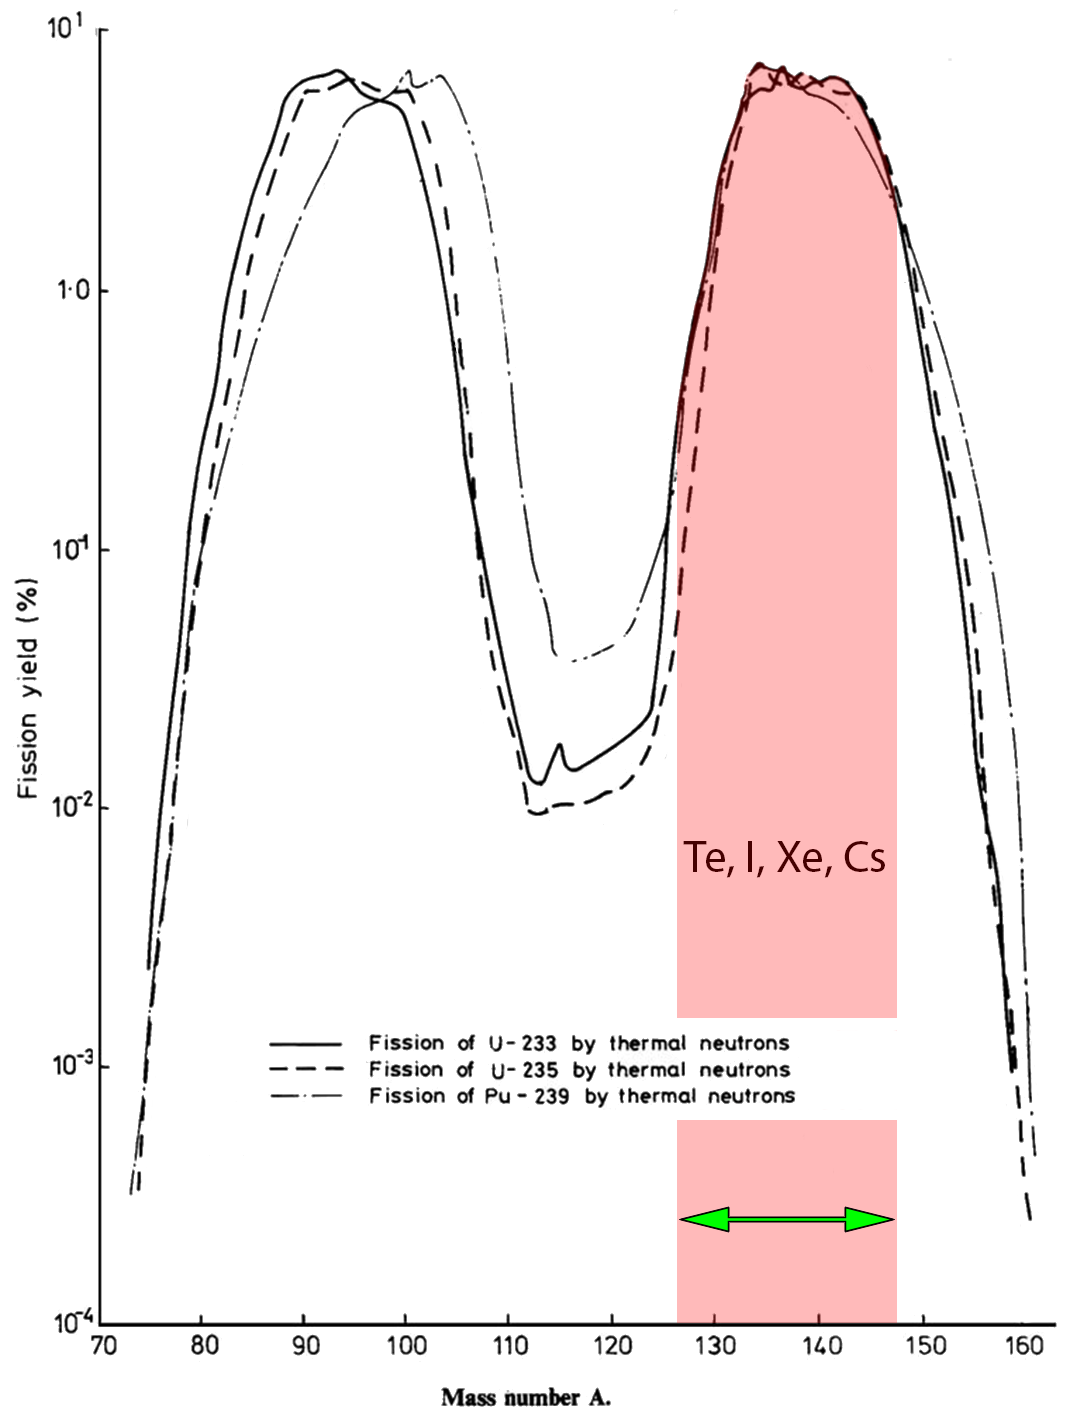
\includegraphics[height=11cm]{images/fissionyield.png}
    \caption[Plot of the percentage yield of nuclei with a given mass following a fission event. Range of masses corresponding to isotopes of Te, I, Xe and Cs are highlighted.]{Plot of the percentage yield of nuclei with a given mass following a fission event. Range of masses corresponding to isotopes of Te, I, Xe and Cs are highlighted. Adapted from \cite{England1992}.}
    \label{fig:fissionyield}
\end{figure}

Previous work on defect equilibria in \zirconia\ considered the internal oxide layer's effectiveness as a barrier to iodine \cite{kenichiodine2018}. It was found that the tetragonal phase of \zirconia\ is a better barrier to iodine ingress than monoclinic \zirconia , especially at higher oxygen partial pressures. 

Tetragonal \zirconia\ will be present on the inner surface of the cladding because it is self-stabilised by the stresses imposed as the oxide grows into the zirconium metal, in addition to compressive residual stresses induced by radiation damage \cite{causey2005review}. The iodine defect study, however, only informs us about one part of the SCC process. For a more holistic understanding, the life cycle of the iodine must also be taken into account.    

%SCC studies of the internal surface of zirconium-based fuel claddings have been conducted, which indicate that iodine is likely to be one of the main corrosive species involved in promoting crack growth \cite{rosenbaum1966interaction, Cox1990Pellet-cladReview,Fregonese1998AmountIodine,Sidky1998IodineReview}. The exact mechanism for iodine SCC has not yet been determined due to difficulties observing the internal cladding surface in-situ, while experimental studies are not yet capable of reproducing the conditions under which such failures occur. This study focuses on the oxide on the internal surface of the fuel cladding, following from a previous study on iodine in the oxide layer. \\

Nuclei produced during fission are typically neutron-rich, resulting in decay modes such as $\beta-$ or neutron emission. In the case of tellurium nuclei, most decay into iodine, which then decays into xenon with different half-lives depending on the isotope. Several of these isotopes' fission yield and decay data were shown in Table \ref{table:decaydata_chap1}. The decay chain continues with xenon nuclei decaying into caesium, many isotopes of which have half lives measured in years. At this point, conventional power reactor fuel is retired long before a significant proportion of the caesium decays into barium. For this reason, only the elements tellurium through caesium are considered in this study. 

The majority of thermal fission events occur in the outer rim of a fuel pellet. Given a fission product penetration depth of up to 8 $\mu$m in \zirconia\ \cite{degueldre2001behaviour}, a large proportion of fission products implant within the oxide. It has also been observed in PCI failures that there is a highly variable time delay (depending on burnup, fuel power history and ramping rate \cite{international2003iaea}) of up to several hours between the power ramping of the reactor and the subsequent detection of failure of the cladding \cite{bergenlid1980experimental, wood1983effects, pankaskie1981mechanistic}. Figure \ref{figure:BWRrampthreshold} shows cladding failures occurring within 77 minutes following a ramp, whereas figure \ref{figure:fueltests} shows how a cladding failure was detected within 4 hours of a power ramp\footnote{These fuel pins had been irradiated before, but were stored outside a reactor 10 months prior to this test, resulting in a lower fission product inventory than what would normally be present in a real scenario.}. Detection of a cladding failure gives an upper bound for the time delay because it relies on sensors in the core registering the presence of fission products in the coolant. This time delay is in line with the half-lives of many Te and I isotopes (Table \ref{table:decaydata_chap1}) such that significant proportions of these isotopes will decay during this time delay, hinting that these phenomena could be related. 
%In addition, it is known that irradiated cladding containing fresh fuel does not crack when power ramped  \cite{wood1983effects}. \\

With each nuclear decay comes a change in the chemical and therefore physical behaviour of the atom with its immediate environment. For example, an iodine dopant in \zirconia\ may decay into xenon, which may then have a significantly different thermodynamic equilibrium site preference from the one it inherited. Determining the behaviour of each of these elements in the oxide layer may provide information about the initiation of SCC in fuel cladding. A quantum-mechanical calculation approach has therefore been adopted to model the behaviour of the decay chain elements tellurium through caesium within tetragonal phase \zirconia.

\begin{figure}[ht]
    \centering
    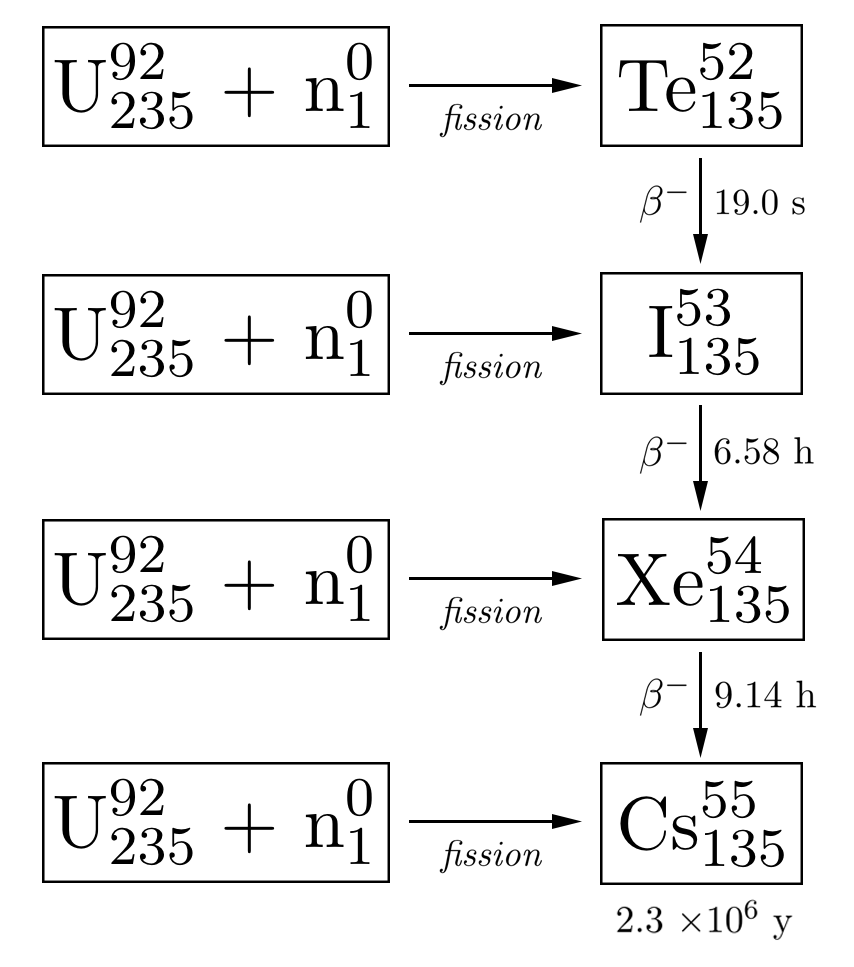
\includegraphics[height=9.5cm]{images/te_decay_chain2.png}
    \caption{Diagram of the production of Te$_{135}$ decay chain elements with decay modes and half-lives shown.}
    \label{fig:decaychain}
\end{figure}

%Iodine is produced in the fuel pellet directly from fission and also from the decay of tellurium precursors. Both iodine and tellurium are relatively common fission products, with combined independent yields from thermal fission of U$_{235}$ above 5\% \cite{kennett1956mass, iodine129fissionyield, imanishi1976independent, iodinefissionyields, iodine132, amiel1975odd}. The majority of thermal fission events occur in the outer rim of the fuel pellet, and a fission product penetration depth of up to 8 $\mu$m in \zirconia\ \cite{degueldre2001behaviour} suggests a large degree of implantation within the oxide and the Zr metal into which the oxide grows, raising the concentration of I well above the equilibrium value. Iodine and many of its compounds (ZrI$_{4}$, CsI) are volatile and fuel pellets contain many cracks and spaces through which iodine may be rapidly transported to the cladding. When reactor power is increased during start-up, iodine is released in substantial quantities from the UO$_{2}$ pellet \cite{peehs1982experimental}. This is believed to cause crack propagation in the cladding when combined with stresses imposed on the cladding by the fuel pellet, a phenomenon known as pellet-cladding interaction (PCI). Upper limits on power ramping and holding times have therefore been established by fuel suppliers to mitigate potential PCI failures \cite{yagnik2005effect}. While these restrictions have reduced or prevented the incidence of PCI failures, they also impose costs on the operator due to longer ramping periods. This also restricts the ability of the nuclear reactor to load-follow grid demand. Cladding/fuel materials resistant to PCI failure are therefore of great interest in the nuclear power industry, promoting research into solutions such as cladding liners and doped fuel pellets \cite{nonon2005pci,yang2012effect}. \\

%\item Power ramping: Increasing power, such as during reactor start-up, can lead to cladding failure.   %power must be ramped up gradually in order to avoid excessive temperature gradients in the fuel pins, but also to manage fission product concentrations. Due to the different half-lives of various fission products, a power ramp will cause a transient increase in the iodine concentration within a fuel pin


%Iodine is an oxidising agent, which, under standard conditions, will oxidise Zr metal to produce ZrI$_{4}$. However, oxygen is also present in the internal fuel pin environment, both from the native \zirconia\ layer on the cladding, and the evolution of oxygen from the fuel pellet during burnup. Liberated oxygen will compete with iodine in the oxidation of the Zr metal, but whereas iodine promotes crack growth under stress, oxygen provides a more protective effect, self-limiting its diffusion into the metal \cite{farina2002stress, causey2005review}. Furthermore, oxygen is a more powerful oxidising agent than iodine, reacting together to produce I${_2}$O$_{5}$. For these reasons, the internal oxide layer of the cladding is often considered a barrier to the ingress of iodine into the Zr metal. \\

%Unlike oxygen and hydrogen, which readily diffuse into Zr metal to occupy interstitial sites, iodine atoms have been predicted in atomistic studies to have very high energy barriers to bulk interstitial diffusion \cite{rossi2015first,legris2005ab,carlot2002energetically}. This is due to the relatively large radius of the iodine atom, which imposes large local strains when penetrating the Zr lattice. This suggests that iodine will instead be transported towards crack tips via grain boundaries. Indeed, intergranular cracking has been observed in PCI failures, but only for a few hundred nm before a more rapid transgranular crack propagation \cite{fregonese2000failure}. Conversely, no atomic scale studies of iodine in \zirconia\ were found in the literature.  \\

%\zirconia\ grown thermally on Zr metal exists mainly in either the monoclinic or tetragonal phase \cite{Howard1988StructuresDiffraction,teufer1962crystal}. We can expect the internal \zirconia\ layer of the cladding to be mostly monoclinic in early life, with the stress-stabilised tetragonal phase appearing near the oxide/metal interface due to cohesive strains resulting from the lattice mismatch. With increasing burnup however, it is expected that more tetragonal and possibly even the cubic phase of \zirconia\ forms due to vacancy formation and residual stresses in the lattice from radiation damage \cite{sickafus1999radiation}. Amorphisation due to radiation damage has also been observed in the cubic phase from Cs$^{+}$ implantation \cite{amorphization2000wang}. In this study however, while defect energies for the cubic phase are reported, we focus our analysis on monoclinic and tetragonal \zirconia\ phases, partly due to difficulties predicting the behaviour of the pure high-temperature cubic phase using energies calculated from a static energy technique. \\

%The effectiveness of the oxide layer as a barrier to iodine is debated, with one study presuming that the oxide is bypassed entirely by iodine due to fracturing, leaving the Zr metal underneath exposed \cite{rossi2015first}. The outermost part of the oxide, which is porous, exhibits networks of interconnected grain boundary diffusion pathways towards the oxide/metal interface which are certainly wide enough (1-3 nm) to allow iodine transport \cite{ni2010porosity}. The oxygen-saturated Zr at the oxide/metal interface is not, however, taken into account, and it is expected that this will influence the corrosion mechanism due to iodine-oxygen competition: even the much smaller hydrogen atom has its rate of diffusion into the metal reduced by the presence of oxygen, as shown in both computational \cite{glazoff2014oxidation} and experimental hydrogen pick-up studies \cite{couet2014hydrogen}. This means that some barrier to iodine ingress must already exist near the oxide/metal interface. The varying levels of oxygen across the oxide layer itself also have an effect on defect behaviour, and will therefore influence the initiation mechanisms behind PCI failures. Thus here, we predict iodine incorporation energies and defect equilibria in \zirconia\ as a function of oxygen pressure through Brouwer diagrams, in order to predict the resulting iodine defect response.

\section{\label{Method}Methodology}

\subsection{Computational Parameters}

Calculations were performed using the CASTEP 8.0 density functional theory (DFT) based code \cite{Clark2005}. Ultra-soft pseudo-potentials with a cut-off energy of 600 eV were employed. The Perdew, Burke and Ernzerhof (PBE) \cite{Perdew1996} parameterisation of the generalised gradient approximation (GGA) was used to describe the exchange correlation functional. A Monkhorst-Pack sampling scheme \cite{Monkhorst1976} was used for Brillouin zone integration, with a minimum \emph{k}-point separation of 0.09 \r{A}\textsuperscript{-1}. The Pulay method for density mixing \cite{Pulay1980} was used to improve simulation convergence. 

The electronic energy convergence criterion was set to $1\times10^{-6}$ eV and the maximum force between atoms limited to $1\times10^{-2}$ eV \r{A}\textsuperscript{-1}. A gradient-descent geometry optimisation task was run on the cell until consecutive iterations differed in energy and atomic displacement by less than $1\times10^{-5}$ eV and $5\times10^{-4}$ \r{A} respectively. 

Using these convergence criteria, non-defective supercells of tetragonal (3x3x2 unit cells) \zirconia\ were relaxed under constant pressure. The resulting structure was used as the starting point to which defects were introduced, and subsequently relaxed again, this time under constant volume conditions to simulate low defect concentrations \cite{Murphy2014, Bell2015}. The supercell was constructed such that its dimensions were as close to a cube as possible in order to minimise directional defect self-interaction across the periodic boundaries. 


\subsection{Defect Volumes}

As described in § \ref{isobaricmethod}, defect volumes were calculated by completely relaxing an unconstrained, defective supercell using the geometry optimisation task in CASTEP. This allows the defective supercell to alter its volume in order to minimise the total energy of the system, at which point this `optimal' supercell volume is recorded. The non-defective supercell volume, calculated in the same way, is then subtracted from the defective supercell volume to give the individual defect volume.

\subsection{Defect Equilibrium Response to Oxygen Partial Pressure}

Brouwer diagrams, also known as Kr{\"o}ger-Vink diagrams, were produced using a method outlined by Murphy et al. \cite{Murphy2014a} to determine defect concentrations as a function of oxygen partial pressure. We start from the statement that the chemical potential of \zirconia\ is equivalent to the sum of the chemical potentials $\mu$ of its constituent species, Zr and O:

\begin{equation}
{\mu}_{ZrO_2(s)} = {\mu}_{Zr}(p_{O_2}, T) + {\mu}_{O_2}(p_{O_2}, T)
\label{mewZrO2}
\end{equation}

where $T$ denotes temperature and $p_{O_2}$ denotes oxygen partial pressure. The chemical potential of \zirconia\ in the solid state is assumed to have negligible dependence on $T$ and $p_{O_2}$ relative to ${\mu}_{Zr}$ and ${\mu}_{O_2}$. Energies can be obtained for bulk \zirconia\ and Zr, but the ground state of oxygen is not correctly reproduced in DFT \cite{Batyrev2000, Lozovoi2001}. Instead, we use the approach of Finnis et al. \cite{Finnis2005} to infer the oxygen chemical potential from standard state values. We can use the experimental Gibbs free energy to produce an equation where $\mu_{O_2}$ is the only unknown:
\begin{equation}
\Delta{G^{\plimsoll}_{f, ZrO_2}} = \mu_{ZrO_2(s)} - (\mu_{Zr(s)} + \mu^{\plimsoll}_{O_2})
\end{equation}

where $\Delta{G^{\plimsoll}_{f, ZrO_2}}$ is the experimental Gibbs energy at standard temperature and pressure and $\mu^{\plimsoll}_{O_2}$ is the oxygen chemical potential under the same conditions. The values of $\mu_{ZrO_2(s)}$ and $\mu_{Zr(s)}$ are calculated from the DFT energies. Once $\mu^{\plimsoll}_{O_2}$ is calculated, we can generalise the chemical potential of oxygen for any value of $T$ and $p_{O_2}$ by appending an ideal gas relationship $\Delta{\mu(T)}$ and a Boltzmann distribution:

\begin{equation}
\mu_{O_2}(p_{O_2},T) = \mu^{\plimsoll}_{O_2} + \Delta{\mu(T)} + \frac{1}{2}{k_B}log(\frac{p_{O_2}}{p^{\plimsoll}_{O_2}})
\end{equation}

Using our generalised formula for $\mu_{O_2}$, we fix the temperature within the range of thermal phase-stabilisation (1500 K for tetragonal \zirconia) and calculate $\mu_{O_2}$ for many different values of $p_{O_2}$ between $10^{-35}$ and 10$^{0}$ atm, corresponding to oxygen deficient and oxygen rich environments, respectively ($p_{O_2}$ in air is approximately 0.2 atm). While the tetragonal phase will be stress-stabilised in practice, thermal-stabilisation in such models has been shown to qualitatively approximate the effect of stress-stabilisation, while allowing a wider range of dopant behaviours to be predicted \cite{Bell2016}. Equilibrium defect concentrations are then calculated at each $\mu_{O_2}$ and plotted against $p_{O_2}$ to produce a Brouwer diagram. Brouwer diagrams at extrinsic defect concentrations of $10^{-5}$ and $10^{-3}$ parts/fu (i.e. parts per \zirconia\ formula unit) were generated to examine low and high dopant concentrations, respectively. These two concentrations were examined because the amount of fission products present at a particular point in a fuel pellet depends on macroscopic parameters, including its position in the core and the time since the last shutdown, but also microscopic parameters such as the radial position in the pellet. %These two concentrations were selected because $10^{-3}$ parts/fu is high enough to model an aggregation of iodine (such as at a crack tip), and $10^{-5}$ parts/fu was found to be the concentration below which iodine did not have a significant effect on defect equilibria. 

\section{Results} \label{Results}

\subsection{Brouwer Diagrams}

\subsubsection{Tellurium}

Brouwer diagrams for tellurium defects are shown in Figure \ref{figure:telluriumbrouwer}. At a tellurium defect concentration of $10^{-5}$ parts per f.u. \zirconia , the dominant defect was \ch{Te_{O}^{**}} over the oxygen pressure range of $10^{-28}$ to $10^{-7}$ atm. This is mainly charge compensated by intrinsic electronic defects at lower oxygen pressures, and zirconium vacancies at higher oxygen pressures. At higher oxygen pressures, tellurium preferentially occupies zirconium sites, producing the defect \ch{Te_{Zr}^{'''}}, this time charge compensated by positive hole defects. 

\begin{figure}[htp] % Tellurium 1
\begin{center}
\begin{tikzpicture}
	\begin{groupplot}[group style={group size=1 by 2}, width=14cm, height=11cm]
	\nextgroupplot[
		 ylabel={\ch{log_{10}}([D]) (per f.u.)}, ymin=-10, ymax=0, xmin=-35, xmax=0, legend style={{draw=}, at={(0.40,0.97)}, anchor=north west, legend columns=4, nodes={scale=1, transform shape}}]
        \addplot[no marks, draw=blue!70!black] table [x=pO2, y=electrons,]{dat/te_tet_10-5.dat}; \addlegendentry{\ch{e^{'}}}; \node at (-26.0,-1.9) {\ch{e^{'}}};
        \addplot[no marks, draw=red!85!black] table [x=pO2, y=holes,]{dat/te_tet_10-5.dat}; \addlegendentry{\ch{h^{\textperiodcentered}}}; \node at (-7,-3.6) {\ch{h^{\textperiodcentered}}};
        \addplot[no marks, draw=black!70!green] table [x=pO2, y=VO{2},]{dat/te_tet_10-5.dat}; \addlegendentry{\ch{V_{O}^{\textperiodcentered\textperiodcentered}}}; \node at (-26.7,-3.3) {\ch{V_{O}^{\textperiodcentered\textperiodcentered}}};
         %\addplot[no marks, draw=black!55!green] table [x=pO2, y=VO{1},]{dat/te_tet_10-5.dat}; \addlegendentry{\ch{V_{O}^{\textperiodcentered}}};
         %\addplot[no marks, draw=black!30!green] table [x=pO2, y=VO{0},]{dat/te_tet_10-5.dat}; \addlegendentry{\ch{V_{O}^{x}}};
        \addplot[no marks, draw=yellow!85!blue] table [x=pO2, y=VM{-4},]{dat/te_tet_10-5.dat}; \addlegendentry{\ch{V_{Zr}^{''''}}};
         %\addplot[no marks, draw=yellow!75!blue] table [x=pO2, y=VM{-3},]{dat/te_tet_10-5.dat}; \addlegendentry{\ch{V_{Zr}^{'''}}};
         %\addplot[no marks, draw=yellow!65!blue] table [x=pO2, y=VM{-2},]{dat/te_tet_10-5.dat}; \addlegendentry{\ch{V_{Zr}^{''}}};
         %\addplot[no marks, draw=yellow!55!blue] table [x=pO2, y=VM{-1},]{dat/te_tet_10-5.dat}; \addlegendentry{\ch{V_{Zr}^{'}}};
         %\addplot[no marks, draw=yellow!45!blue] table [x=pO2, y=VM{0},]{dat/te_tet_10-5.dat}; \addlegendentry{\ch{V_{Zr}^{x}}};
         %\addplot[no marks, draw=red!60!yellow] table [x=pO2, y=Oi{-2},]{dat/te_tet_10-5.dat}; \addlegendentry{\ch{O_{i}^{''}}};
         %\addplot[no marks, draw=red!50!yellow] table [x=pO2, y=Oi{-1},]{dat/te_tet_10-5.dat}; \addlegendentry{\ch{O_{i}^{'}}};
         %\addplot[no marks, draw=red!40!yellow] table [x=pO2, y=Oi{0},]{dat/te_tet_10-5.dat}; \addlegendentry{\ch{O_{i}^{x}}};
         %\addplot[no marks, draw=green!80!pink] table [x=pO2, y=Mi{4},]{dat/te_tet_10-5.dat}; \addlegendentry{\ch{Zr_{i}^{\textperiodcentered\textperiodcentered\textperiodcentered\textperiodcentered}}};
         %\addplot[no marks, draw=green!70!pink] table [x=pO2, y=Mi{3},]{dat/te_tet_10-5.dat}; \addlegendentry{\ch{Zr_{i}^{\textperiodcentered\textperiodcentered\textperiodcentered}}};
         %\addplot[no marks, draw=green!60!pink] table [x=pO2, y=Mi{2},]{dat/te_tet_10-5.dat}; \addlegendentry{\ch{Zr_{i}^{\textbf{\textperiodcentered\textperiodcentered}}}};
        %\addplot[no marks, draw=green!50!pink] table [x=pO2, y=Mi{1},]{dat/te_tet_10-5.dat}; \addlegendentry{\ch{Zr_{i}^{\textperiodcentered}}};
         %\addplot[no marks, draw=green!40!pink] table [x=pO2, y=Mi{0},]{dat/te_tet_10-5.dat}; \addlegendentry{\ch{Zr_{i}^{x}}};
         %\addplot[no marks, dashed, draw=red!70!black] table [x=pO2, y=Tei{0},]{dat/te_tet_10-5.dat}; \addlegendentry{\ch{Te_{i}^{x}}};
         %\addplot[no marks, dashed, draw=red!50!black] table [x=pO2, y=Tei{-1},]{dat/te_tet_10-5.dat}; \addlegendentry{\ch{Te_{i}^{'}}};
        %\addplot[no marks, dashed, draw=purple] table [x=pO2, y=Tei{1},]{dat/te_tet_10-5.dat}; \addlegendentry{\ch{Te_{i}^{\textperiodcentered}}};
        \addplot[no marks, dashed, draw=blue!50!white] table [x=pO2, y=TesubO{1},]{dat/te_tet_10-5.dat}; \addlegendentry{\ch{Te_{O}^{\textperiodcentered}}};
        \addplot[no marks, dashed, draw=green!60!black] table [x=pO2, y=TesubO{2},]{dat/te_tet_10-5.dat}; \addlegendentry{\ch{Te_{O}^{\textperiodcentered\textperiodcentered}}};
        %\addplot[no marks, dashed, draw=black] table [x=pO2, y=TesubO{3},]{dat/te_tet_10-5.dat}; \addlegendentry{\ch{Te_{O}^{\textperiodcentered\textperiodcentered\textperiodcentered}}};
        \addplot[no marks, dashed, draw=orange!80!black] table [x=pO2, y=TesubZr{-3},]{dat/te_tet_10-5.dat}; \addlegendentry{\ch{Te_{Zr}^{'''}}};
         %\addplot[no marks, dashed, draw=pink] table [x=pO2, y=TesubZr{-4},]{dat/te_tet_10-5.dat}; \addlegendentry{\ch{Te_{Zr}^{''''}}};
         %\addplot[no marks, dashed, draw=purple] table [x=pO2, y=TesubZr{-5},]{dat/te_tet_10-5.dat}; \addlegendentry{\ch{Te_{Zr}^{'''''}}};
%         \addplot[no marks] table [x=pO2, y=Stoich,]{cs_tet.dat}; \addlegendentry{Stoich};
\node at (-33.7,-0.5) {\textbf{a)}};
			\nextgroupplot[
		 xlabel={\ch{log_{10}}($p_{O_{2}}$) (atm)}, ylabel={\ch{log_{10}}([D]) (per f.u.)}, ymin=-10, ymax=0, xmin=-35, xmax=0, legend style={{draw=}, at={(0.40,0.97)}, anchor=north west, legend columns=4, nodes={scale=1, transform shape}}]
        \addplot[no marks, draw=blue!70!black] table [x=pO2, y=electrons,]{dat/te_tet_10-3.dat}; \node at (-27,-1.7) {\ch{e^{'}}};
        \addplot[no marks, draw=red!85!black] table [x=pO2, y=holes,]{dat/te_tet_10-3.dat}; %\node at (-2.5,-2.1) {\ch{h^{\textperiodcentered}}};
        \addplot[no marks, draw=black!70!green] table [x=pO2, y=VO{2},]{dat/te_tet_10-3.dat}; 
         %\addplot[no marks, draw=black!55!green] table [x=pO2, y=VO{1},]{dat/te_tet_10-3.dat}; 
         %\addplot[no marks, draw=black!30!green] table [x=pO2, y=VO{0},]{dat/te_tet_10-3.dat}; 
        \addplot[no marks, draw=yellow!85!blue] table [x=pO2, y=VM{-4},]{dat/te_tet_10-3.dat}; 
%         \addplot[no marks, draw=yellow!75!blue] table [x=pO2, y=VM{-3},]{dat/te_tet_10-3.dat}; 
%         \addplot[no marks, draw=yellow!65!blue] table [x=pO2, y=VM{-2},]{dat/te_tet_10-3.dat}; 
%         \addplot[no marks, draw=yellow!55!blue] table [x=pO2, y=VM{-1},]{dat/te_tet_10-3.dat}; 
%         \addplot[no marks, draw=yellow!45!blue] table [x=pO2, y=VM{0},]{dat/te_tet_10-3.dat}; 
%         \addplot[no marks, draw=red!60!yellow] table [x=pO2, y=Oi{-2},]{dat/te_tet_10-3.dat}; 
%         \addplot[no marks, draw=red!50!yellow] table [x=pO2, y=Oi{-1},]{dat/te_tet_10-3.dat}; 
%         \addplot[no marks, draw=red!40!yellow] table [x=pO2, y=Oi{0},]{dat/te_tet_10-3.dat}; 
%         \addplot[no marks, draw=green!80!pink] table [x=pO2, y=Mi{4},]{dat/te_tet_10-3.dat}; 
%         \addplot[no marks, draw=green!70!pink] table [x=pO2, y=Mi{3},]{dat/te_tet_10-3.dat}; 
%         \addplot[no marks, draw=green!60!pink] table [x=pO2, y=Mi{2},]{dat/te_tet_10-3.dat}; 
%         \addplot[no marks, draw=green!50!pink] table [x=pO2, y=Mi{1},]{dat/te_tet_10-3.dat}; 
%         \addplot[no marks, draw=green!40!pink] table [x=pO2, y=Mi{0},]{dat/te_tet_10-3.dat}; 
        %\addplot[no marks, dashed, draw=red!70!black] table [x=pO2, y=Tei{0},]{dat/te_tet_10-3.dat}; 
        %\addplot[no marks, dashed, draw=red!50!black] table [x=pO2, y=Tei{-1},]{dat/te_tet_10-3.dat}; 
        %\addplot[no marks, dashed, draw=purple] table [x=pO2, y=Tei{1},]{dat/te_tet_10-3.dat}; 
        \addplot[no marks, dashed, draw=blue!50!white] table [x=pO2, y=TesubO{1},]{dat/te_tet_10-3.dat}; 
        \addplot[no marks, dashed, draw=green!60!black] table [x=pO2, y=TesubO{2},]{dat/te_tet_10-3.dat}; \node at (-11,-2.6) {\ch{Te_{O}^{\textperiodcentered\textperiodcentered}}};
        %\addplot[no marks, dashed, draw=black] table [x=pO2, y=TesubO{3},]{dat/te_tet_10-3.dat}; 
        \addplot[no marks, dashed, draw=orange!80!black] table [x=pO2, y=TesubZr{-3},]{dat/te_tet_10-3.dat}; 
        %\addplot[no marks, dashed, draw=pink] table [x=pO2, y=TesubZr{-4},]{dat/te_tet_10-3.dat}; 
        %\addplot[no marks, dashed, draw=purple] table [x=pO2, y=TesubZr{-5},]{dat/te_tet_10-3.dat}; 
%        \addplot[no marks] table [x=pO2, y=Stoich,]{dat/te_tet_10-3.dat}; 
\node at (-33.7,-0.5) {\textbf{b)}};
			\end{groupplot}           
\end{tikzpicture}
		\caption{Brouwer diagrams for tetragonal phase \zirconia\ point defects at tellurium concentrations of a) $10^{-5}$ and b) $10^{-3}$, at a temperature of 1500 K.} % Space charge = 0
		\label{figure:telluriumbrouwer}
	\end{center}
\end{figure}

Tellurium on an oxygen site adopts a 0 charge state, which while not obvious (it may be expected to act like oxygen, also a group 6 element), can be understood when considering chemical behaviour. Oxygen on its native site will readily adopt a charge state of -2. Tellurium on the other hand, exhibits more metallic behaviour, preferring to be oxidised itself (the electronegativities of oxygen and tellurium are 3.5 and 2.1 respectively). However, the \ch{V_{O}^{**}} site is highly reducing, and will counter the tellurium ion's proclivity to oxidise. The overall effect on tellurium in this case is to maintain its original electronic structure. Finally, when the tellurium concentration is increased to $10^{-3}$ parts/fu, greater occupancy on the zirconium site is predicted above oxygen pressures of $10^{-17}$ atm, forming the defect \ch{Te_{Zr}^{'''}}. This corresponds to a tellurium charge state of +1. While an even more positive charge state for tellurium would normally be expected, in this case it is the dominant negative defect by an order of magnitude and is necessary to provide charge compensation for positive hole and \ch{Te_{O}^{**}} defects. 

The presence of these defects and their sizes will have an effect on the lattice, particularly if there is a lattice mismatch which results in a significant local strain. In terms of defect volume, \ch{Te_{O}^{**}} has a slightly positive volume of 2.74 \r{A}$^{3}$ relative to the non-defective crystal. This is quite large for a positively charged defect (\ch{V_{O}^{**}} has a defect volume of -40.45 \r{A}$^{3}$), very likely due to the large size of the tellurium atom itself. When tellurium occupies the zirconium site, the resulting \ch{Te_{Zr}^{'''}} has a defect volume of 59.93 \r{A}$^{3}$. While this is lower than the defect volume of \ch{V_{Zr}^{''''}} (88.93 \r{A}$^{3}$), it is still an increase in volume relative to the non-defective crystal and will impart a strain on the lattice which, at a high enough defect concentration, could contribute to crack formation.

\subsubsection{Iodine}

Iodine was previously predicted in Brouwer diagrams (Figure \ref{figure:tikzbrouwerconctet} to produce the defects \ch{I_{O}^{*}} and \ch{I_{Zr}^{'''}} at low and high oxygen pressures respectively. Since the extrinsic defect site is similar for tellurium defects over most oxygen pressures, $\beta$- decay of tellurium could have directly produced these iodine defects without requiring a change of site. Thus, \ch{Te_{O}^{**}} would decay and produce \ch{I_{O}^{*}} with a defect volume of 29.90 \r{A}$^{3}$, and \ch{Te_{Zr}^{'''}} would decay and produce \ch{I_{Zr}^{'''}} with a defect volume of 87.07 \r{A}$^{3}$. At the oxygen site, this means a defect volume change from 2.74 to 29.90 \r{A}$^{3}$. This increase is in large part due to the change in charge state from 0 to -1, as the ions are of similar size otherwise. 

Similarly at the zirconium site, the defect volume changes from 59.93 to 87.07 \r{A}$^{3}$. Both of these are relatively large increases in defect volume and will come with an increase in lattice stress in the immediate vicinity of the defect, especially if highly constrained. Of course, this  process will take place continuously over time as tellurium atoms decay, with half-lives ranging from seconds to hours depending on the isotope. It is of note however, that PCI failures tend to occur after power ramps with a time delay, ranging from several minutes to hours after the transient. While not conclusive, this may hint at a mechanism involving decay processes. 

%%-----Brouwer Diagram Iodine-----%
%\begin{landscape}
%\begin{figure}[ht] % Iodine
%\begin{center}
%\begin{tikzpicture}
%	\begin{axis}
%		[width=12.35cm, xlabel={\ch{log_{10}}($p_{O_{2}}$) (atm)}, ylabel={\ch{log_{10}}([D]) (per f.u.)}, ymin=-10, ymax=0, xmin=-35, xmax=0, legend style={{draw=}, at={(0.40,0.97)}, anchor=north west, legend columns=3, nodes={scale=0.75, transform shape}}]
%        \addplot[no marks, draw=blue!70!black] table [x=pO2, y=electrons,]{dat/1e5iconctet1500.dat}; \addlegendentry{\ch{e^{'}}}; \node at (-26.0,-1.9) {\ch{e^{'}}};
%        \addplot[no marks, draw=red!85!black] table [x=pO2, y=holes,]{dat/1e5iconctet1500.dat}; \addlegendentry{\ch{h^{\textperiodcentered}}}; \node at (-7,-3.6) {\ch{h^{\textperiodcentered}}};
%        \addplot[no marks, draw=black!70!green] table [x=pO2, y=VO{2},]{dat/1e5iconctet1500.dat}; \addlegendentry{\ch{V_{O}^{\textperiodcentered\textperiodcentered}}}; \node at (-26.7,-3.3) {\ch{V_{O}^{\textperiodcentered\textperiodcentered}}};
%%         \addplot[no marks, draw=black!55!green] table [x=pO2, y=VO{1},]{dat/1e5iconctet1500.dat}; \addlegendentry{\ch{V_{O}^{\textperiodcentered}}};
%%         \addplot[no marks, draw=black!30!green] table [x=pO2, y=VO{0},]{dat/1e5iconctet1500.dat}; \addlegendentry{\ch{V_{O}^{x}}};
%        \addplot[no marks, draw=yellow!85!blue] table [x=pO2, y=VM{-4},]{dat/1e5iconctet1500.dat}; \addlegendentry{\ch{V_{Zr}^{''''}}};
%%         \addplot[no marks, draw=yellow!75!blue] table [x=pO2, y=VM{-3},]{dat/1e5iconctet1500.dat}; \addlegendentry{\ch{V_{Zr}^{'''}}};
%%         \addplot[no marks, draw=yellow!65!blue] table [x=pO2, y=VM{-2},]{dat/1e5iconctet1500.dat}; \addlegendentry{\ch{V_{Zr}^{''}}};
%%         \addplot[no marks, draw=yellow!55!blue] table [x=pO2, y=VM{-1},]{dat/1e5iconctet1500.dat}; \addlegendentry{\ch{V_{Zr}^{'}}};
%%         \addplot[no marks, draw=yellow!45!blue] table [x=pO2, y=VM{0},]{dat/1e5iconctet1500.dat}; \addlegendentry{\ch{V_{Zr}^{x}}};
%%         \addplot[no marks, draw=red!60!yellow] table [x=pO2, y=Oi{-2},]{dat/1e5iconctet1500.dat}; \addlegendentry{\ch{O_{i}^{''}}};
%%         \addplot[no marks, draw=red!50!yellow] table [x=pO2, y=Oi{-1},]{dat/1e5iconctet1500.dat}; \addlegendentry{\ch{O_{i}^{'}}};
%%         \addplot[no marks, draw=red!40!yellow] table [x=pO2, y=Oi{0},]{dat/1e5iconctet1500.dat}; \addlegendentry{\ch{O_{i}^{x}}};
%%         \addplot[no marks, draw=green!80!pink] table [x=pO2, y=Mi{4},]{dat/1e5iconctet1500.dat}; \addlegendentry{\ch{Zr_{i}^{\textperiodcentered\textperiodcentered\textperiodcentered\textperiodcentered}}};
%%         \addplot[no marks, draw=green!70!pink] table [x=pO2, y=Mi{3},]{dat/1e5iconctet1500.dat}; \addlegendentry{\ch{Zr_{i}^{\textperiodcentered\textperiodcentered\textperiodcentered}}};
%%         \addplot[no marks, draw=green!60!pink] table [x=pO2, y=Mi{2},]{dat/1e5iconctet1500.dat}; \addlegendentry{\ch{Zr_{i}^{\textbf{\textperiodcentered\textperiodcentered}}}};
%%         \addplot[no marks, draw=green!50!pink] table [x=pO2, y=Mi{1},]{dat/1e5iconctet1500.dat}; \addlegendentry{\ch{Zr_{i}^{\textperiodcentered}}};
%%         \addplot[no marks, draw=green!40!pink] table [x=pO2, y=Mi{0},]{dat/1e5iconctet1500.dat}; \addlegendentry{\ch{Zr_{i}^{x}}};
%%         \addplot[no marks, dashed, draw=red!70!black] table [x=pO2, y=Ii{0},]{dat/1e5iconctet1500.dat}; \addlegendentry{\ch{I_{i}^{x}}};
%%         \addplot[no marks, dashed, draw=red!50!black] table [x=pO2, y=Ii{-1},]{dat/1e5iconctet1500.dat}; \addlegendentry{\ch{I_{i}^{'}}};
%        \addplot[no marks, dashed, draw=purple!60!white] table [x=pO2, y=Ii{1},]{dat/1e5iconctet1500.dat}; \addlegendentry{\ch{I_{i}^{\textperiodcentered}}};
%        \addplot[no marks, dashed, draw=blue!50!white] table [x=pO2, y=IsubO{1},]{dat/1e5iconctet1500.dat}; \addlegendentry{\ch{I_{O}^{\textperiodcentered}}};
%        \addplot[no marks, dashed, draw=green!60!black] table [x=pO2, y=IsubO{2},]{dat/1e5iconctet1500.dat}; \addlegendentry{\ch{I_{O}^{\textperiodcentered\textperiodcentered}}};
%        \addplot[no marks, dashed, draw=black] table [x=pO2, y=IsubO{3},]{dat/1e5iconctet1500.dat}; \addlegendentry{\ch{I_{O}^{\textperiodcentered\textperiodcentered\textperiodcentered}}};
%        \addplot[no marks, dashed, draw=orange!80!black] table [x=pO2, y=IsubZr{-3},]{dat/1e5iconctet1500.dat}; \addlegendentry{\ch{I_{Zr}^{'''}}};
%%         \addplot[no marks, dashed, draw=pink] table [x=pO2, y=IsubZr{-4},]{dat/1e5iconctet1500.dat}; \addlegendentry{\ch{I_{Zr}^{''''}}};
%%         \addplot[no marks, dashed, draw=purple] table [x=pO2, y=IsubZr{-5},]{dat/1e5iconctet1500.dat}; \addlegendentry{\ch{I_{Zr}^{'''''}}};
%%         \addplot[no marks] table [x=pO2, y=Stoich,]{dat/1e5iconctet1500.dat}; \addlegendentry{Stoich};
%\node at (-33.7,-0.5) {\textbf{a)}};
%			\end{axis}            
%\end{tikzpicture}
%\begin{tikzpicture} % Iodine 2
%	\begin{axis}
%		[width=12.35cm, xlabel={\ch{log_{10}}($p_{O_{2}}$) (atm)}, yticklabels={}, ymin=-10, ymax=0, xmin=-35, xmax=0]
%        \addplot[no marks, draw=blue!70!black] table [x=pO2, y=electrons,]{dat/1e3iconctet1500.dat}; \node at (-27,-1.7) {\ch{e^{'}}};
%        \addplot[no marks, draw=red!85!black] table [x=pO2, y=holes,]{dat/1e3iconctet1500.dat}; \node at (-2.5,-2.1) {\ch{h^{\textperiodcentered}}};
%        \addplot[no marks, draw=black!70!green] table [x=pO2, y=VO{2},]{dat/1e3iconctet1500.dat}; 
%%         \addplot[no marks, draw=black!55!green] table [x=pO2, y=VO{1},]{dat/1e3iconctet1500.dat}; 
%%         \addplot[no marks, draw=black!30!green] table [x=pO2, y=VO{0},]{dat/1e3iconctet1500.dat}; 
%        \addplot[no marks, draw=yellow!85!blue] table [x=pO2, y=VM{-4},]{dat/1e3iconctet1500.dat}; 
%%         \addplot[no marks, draw=yellow!75!blue] table [x=pO2, y=VM{-3},]{dat/1e3iconctet1500.dat}; 
%%         \addplot[no marks, draw=yellow!65!blue] table [x=pO2, y=VM{-2},]{dat/1e3iconctet1500.dat}; 
%%         \addplot[no marks, draw=yellow!55!blue] table [x=pO2, y=VM{-1},]{dat/1e3iconctet1500.dat}; 
%%         \addplot[no marks, draw=yellow!45!blue] table [x=pO2, y=VM{0},]{dat/1e3iconctet1500.dat}; 
%%         \addplot[no marks, draw=red!60!yellow] table [x=pO2, y=Oi{-2},]{dat/1e3iconctet1500.dat}; 
%%         \addplot[no marks, draw=red!50!yellow] table [x=pO2, y=Oi{-1},]{dat/1e3iconctet1500.dat}; 
%%         \addplot[no marks, draw=red!40!yellow] table [x=pO2, y=Oi{0},]{dat/1e3iconctet1500.dat}; 
%%         \addplot[no marks, draw=green!80!pink] table [x=pO2, y=Mi{4},]{dat/1e3iconctet1500.dat}; 
%%         \addplot[no marks, draw=green!70!pink] table [x=pO2, y=Mi{3},]{dat/1e3iconctet1500.dat}; 
%%         \addplot[no marks, draw=green!60!pink] table [x=pO2, y=Mi{2},]{dat/1e3iconctet1500.dat}; 
%%         \addplot[no marks, draw=green!50!pink] table [x=pO2, y=Mi{1},]{dat/1e3iconctet1500.dat}; 
%%         \addplot[no marks, draw=green!40!pink] table [x=pO2, y=Mi{0},]{dat/1e3iconctet1500.dat}; 
%%         \addplot[no marks, dashed, draw=red!70!black] table [x=pO2, y=Ii{0},]{dat/1e3iconctet1500.dat}; 
%%         \addplot[no marks, dashed, draw=red!50!black] table [x=pO2, y=Ii{-1},]{dat/1e3iconctet1500.dat}; 
%        \addplot[no marks, dashed, draw=purple!60!white] table [x=pO2, y=Ii{1},]{dat/1e3iconctet1500.dat}; 
%        \addplot[no marks, dashed, draw=blue!50!white] table [x=pO2, y=IsubO{1},]{dat/1e3iconctet1500.dat}; \node at (-11,-2.6) {\ch{I_{O}^{\textperiodcentered}}};
%        \addplot[no marks, dashed, draw=green!60!black] table [x=pO2, y=IsubO{2},]{dat/1e3iconctet1500.dat}; 
%        \addplot[no marks, dashed, draw=black] table [x=pO2, y=IsubO{3},]{dat/1e3iconctet1500.dat}; 
%        \addplot[no marks, dashed, draw=orange!80!black] table [x=pO2, y=IsubZr{-3},]{dat/1e3iconctet1500.dat}; 
%%         \addplot[no marks, dashed, draw=pink] table [x=pO2, y=IsubZr{-4},]{dat/1e3iconctet1500.dat}; 
%%         \addplot[no marks, dashed, draw=purple] table [x=pO2, y=IsubZr{-5},]{dat/1e3iconctet1500.dat}; 
%%         \addplot[no marks] table [x=pO2, y=Stoich,]{dat/1e3iconctet1500.dat}; 
%\node at (-33.7,-0.5) {\textbf{b)}};
%			\end{axis}            
%\end{tikzpicture}
%		\caption{Tetragonal phase Brouwer diagrams of point defects at iodine concentrations of a) $10^{-5}$ and b) $10^{-3}$, at a temperature of 1500 K.}
%		\label{figure:tikzbrouwerconctet_chap7}
%	\end{center}
%\end{figure}
%\end{landscape}

%Brouwer diagrams for the tetragonal phase are shown in Figure \ref{figure:tikzbrouwerconctet}. As these diagrams were generated at a temperature of 1500 K (at which the tetragonal phase becomes stable), intrinsic defect concentrations were significantly higher than in the monoclinic diagrams for all oxygen pressures (though trends remained the same). Intrinsic defects \ch{e^{'}}, \ch{h^{*}}, \ch{V_{O}^{**}} and \ch{V_{Zr}^{''''}} were dominant across most oxygen pressures at an iodine concentration of $10^{-5}$ parts/fu. Only around stoichiometry do extrinsic defect concentrations approach intrinsic values (which as mentioned earlier is why this concentration of iodine was chosen). Across all oxygen pressures, \ch{I_{O}^{*}} and \ch{I_{Zr}^{'''}} are the major iodine defects. Between $10^{-15}$ and $10^{-5}$ atm, Figure \ref{figure:tikzbrouwerconctet} illustrates that the major iodine defect swaps from \ch{I_{O}^{*}} to \ch{I_{Zr}^{'''}}. \\ 

%When the iodine concentration was increased to $10^{-3}$ parts/fu, a significant change in defect equilibria was predicted. The oxygen pressure at stoichiometry increased from $10^{-10}$ to $10^{-6.5}$ atm (for monoclinic \zirconia, it remained at $10^{-7.5}$ atm regardless of iodine concentration). Nevertheless, \ch{I_{O}^{*}} and \ch{I_{Zr}^{'''}} remain the dominant defect pair between oxygen pressures of $10^{-15}$ and $10^{-5}$ atm (as they are at the lower iodine concentration). However, \ch{I_{O}^{*}} and \ch{I_{Zr}^{'''}} became higher concentration defects than both intrinsic \ch{V_{O}^{**}} and \ch{V_{Zr}^{''''}} defects. We also observe that Zr vacancies no longer serve as the main negative charge-compensation defect near stoichiometry, leaving \ch{I_{Zr}^{'''}} as the most energetically favourable negatively-charged defect.  \\

%Unlike in the Brouwer diagrams for the monoclinic phase, for the tetragonal phase, the concentration of iodine substitutional defects on oxygen sites decreases more steeply at high oxygen pressures, peaking near stoichiometry. \ch{I_{O}^{***}} in particular, which was the dominant defect at high oxygen pressures in monoclinic \zirconia , becomes insignificant under the same conditions in the tetragonal phase, with iodine confined to Zr sites. This behaviour is indicative of a `barrier' effect against iodine at high oxygen partial pressures, with oxygen out-competing iodine for oxygen sites. Given that the inner oxide is likely to have a higher tetragonal phase fraction than the external oxide, due to the incorporation of fission products, this result could help to explain why there appears to be an oxygen effect on PCI-related SCC of zirconium alloys \cite{hofmann1984stress}. \\

%Another effect considered was the space charge of the system. Electrons have a higher rate of diffusion than oxygen vacancies in \zirconia , leading to a build-up of oxygen vacancies near the metal-oxide interface as corrosion progresses \cite{bojinov2010influence}. This results in an overall positive charge (since the dominant oxygen vacancy is \ch{V_{O}^{**}} referred to as a space charge. When included in our Brouwer diagrams, this space charge had a negligible effect on the concentration or charge state of iodine up to a charge of $10^{-1}$ holes per f.u. \zirconia . This corresponds to a high concentration of oxygen vacancies relative to the equilibrium concentration, predicting that a significant deviation from the equilibrium is not expected near the metal oxide interface as a result of a positive space charge.

\subsubsection{Xenon}

Brouwer diagrams for xenon defects are shown in Figure \ref{figure:xenonbrouwer}. At a xenon concentration of $10^{-5}$ parts/fu \zirconia , the dominant xenon defect is \ch{Xe_{O}^{**}} at low oxygen pressures, and a combination of \ch{Xe_{O}^{**}}, \ch{Xe_{Zr}^{''''}} and \ch{Xe_{Zr}^{'''}} at stoichiometry ($10^{-9}$ atm) and higher. At a higher xenon concentration of $10^{-3}$ parts/fu \zirconia , \ch{Xe_{O}^{**}} becomes the dominant defect over a greater oxygen pressure range, from $10^{-30}$ to $10^{-5}$ atm, with \ch{Xe_{Zr}^{''''}} also present in high concentrations at oxygen pressures above $10^{-20}$ atm. As a noble gas, it is expected that xenon in a 0 charge state (\ch{Xe_{O}^{**}} and \ch{Xe_{Zr}^{''''}}) will be prevalent since the full electronic shell provides a stable configuration.

\begin{figure}[htp] % XENON
\begin{center}
\begin{tikzpicture}
	\begin{groupplot}[group style={group size=1 by 2}, width=14cm, height=11cm]
	\nextgroupplot[
		 ylabel={\ch{log_{10}}([D]) (per f.u.)}, ymin=-10, ymax=0, xmin=-35, xmax=0, legend style={{draw=}, at={(0.40,0.97)}, anchor=north west, legend columns=4, nodes={scale=1, transform shape}}]
        \addplot[no marks, draw=blue!70!black] table [x=pO2, y=electrons,]{dat/xe_tet_10-5.dat}; \addlegendentry{\ch{e^{'}}}; \node at (-26.0,-1.9) {\ch{e^{'}}};
        \addplot[no marks, draw=red!85!black] table [x=pO2, y=holes,]{dat/xe_tet_10-5.dat}; \addlegendentry{\ch{h^{\textperiodcentered}}}; \node at (-7,-3.6) {\ch{h^{\textperiodcentered}}};
        \addplot[no marks, draw=black!70!green] table [x=pO2, y=VO{2},]{dat/xe_tet_10-5.dat}; \addlegendentry{\ch{V_{O}^{\textperiodcentered\textperiodcentered}}}; \node at (-26.7,-3.3) {\ch{V_{O}^{\textperiodcentered\textperiodcentered}}};
         %\addplot[no marks, draw=black!55!green] table [x=pO2, y=VO{1},]{dat/xe_tet_10-5.dat}; \addlegendentry{\ch{V_{O}^{\textperiodcentered}}};
         %\addplot[no marks, draw=black!30!green] table [x=pO2, y=VO{0},]{dat/xe_tet_10-5.dat}; \addlegendentry{\ch{V_{O}^{x}}};
        \addplot[no marks, draw=yellow!85!blue] table [x=pO2, y=VM{-4},]{dat/xe_tet_10-5.dat}; \addlegendentry{\ch{V_{Zr}^{''''}}};
         %\addplot[no marks, draw=yellow!75!blue] table [x=pO2, y=VM{-3},]{dat/xe_tet_10-5.dat}; \addlegendentry{\ch{V_{Zr}^{'''}}};
         %\addplot[no marks, draw=yellow!65!blue] table [x=pO2, y=VM{-2},]{dat/xe_tet_10-5.dat}; \addlegendentry{\ch{V_{Zr}^{''}}};
         %\addplot[no marks, draw=yellow!55!blue] table [x=pO2, y=VM{-1},]{dat/xe_tet_10-5.dat}; \addlegendentry{\ch{V_{Zr}^{'}}};
         %\addplot[no marks, draw=yellow!45!blue] table [x=pO2, y=VM{0},]{dat/xe_tet_10-5.dat}; \addlegendentry{\ch{V_{Zr}^{x}}};
         %\addplot[no marks, draw=red!60!yellow] table [x=pO2, y=Oi{-2},]{dat/xe_tet_10-5.dat}; \addlegendentry{\ch{O_{i}^{''}}};
         %\addplot[no marks, draw=red!50!yellow] table [x=pO2, y=Oi{-1},]{dat/xe_tet_10-5.dat}; \addlegendentry{\ch{O_{i}^{'}}};
         %\addplot[no marks, draw=red!40!yellow] table [x=pO2, y=Oi{0},]{dat/xe_tet_10-5.dat}; \addlegendentry{\ch{O_{i}^{x}}};
         %\addplot[no marks, draw=green!80!pink] table [x=pO2, y=Mi{4},]{dat/xe_tet_10-5.dat}; \addlegendentry{\ch{Zr_{i}^{\textperiodcentered\textperiodcentered\textperiodcentered\textperiodcentered}}};
         %\addplot[no marks, draw=green!70!pink] table [x=pO2, y=Mi{3},]{dat/xe_tet_10-5.dat}; \addlegendentry{\ch{Zr_{i}^{\textperiodcentered\textperiodcentered\textperiodcentered}}};
         %\addplot[no marks, draw=green!60!pink] table [x=pO2, y=Mi{2},]{dat/xe_tet_10-5.dat}; \addlegendentry{\ch{Zr_{i}^{\textbf{\textperiodcentered\textperiodcentered}}}};
        %\addplot[no marks, draw=green!50!pink] table [x=pO2, y=Mi{1},]{dat/xe_tet_10-5.dat}; \addlegendentry{\ch{Zr_{i}^{\textperiodcentered}}};
         %\addplot[no marks, draw=green!40!pink] table [x=pO2, y=Mi{0},]{dat/xe_tet_10-5.dat}; \addlegendentry{\ch{Zr_{i}^{x}}};
        %\addplot[no marks, dashed, draw=red!70!black] table [x=pO2, y=Xei{0},]{dat/xe_tet_10-5.dat}; \addlegendentry{\ch{Xe_{i}^{x}}};
        %\addplot[no marks, dashed, draw=red!50!black] table [x=pO2, y=Xei{-1},]{dat/xe_tet_10-5.dat}; \addlegendentry{\ch{Xe_{i}^{'}}};
        %\addplot[no marks, dashed, draw=purple] table [x=pO2, y=Xei{1},]{dat/xe_tet_10-5.dat}; \addlegendentry{\ch{Xe_{i}^{\textperiodcentered}}};
        %\addplot[no marks, dashed, draw=blue!50!white] table [x=pO2, y=XesubO{1},]{dat/xe_tet_10-5.dat}; \addlegendentry{\ch{Xe_{O}^{\textperiodcentered}}};
        \addplot[no marks, dashed, draw=orange] table [x=pO2, y=XesubO{2},]{dat/xe_tet_10-5.dat}; \addlegendentry{\ch{Xe_{O}^{\textperiodcentered\textperiodcentered}}};
        %\addplot[no marks, dashed, draw=black] table [x=pO2, y=XesubO{3},]{dat/xe_tet_10-5.dat}; \addlegendentry{\ch{Xe_{O}^{\textperiodcentered\textperiodcentered\textperiodcentered}}};
        \addplot[no marks, dashed, draw=green] table [x=pO2, y=XesubZr{-3},]{dat/xe_tet_10-5.dat}; \addlegendentry{\ch{Xe_{Zr}^{'''}}};
         \addplot[no marks, dashed, draw=blue] table [x=pO2, y=XesubZr{-4},]{dat/xe_tet_10-5.dat}; \addlegendentry{\ch{Xe_{Zr}^{''''}}};
         %\addplot[no marks, dashed, draw=red] table [x=pO2, y=XesubZr{-5},]{dat/xe_tet_10-5.dat}; \addlegendentry{\ch{Xe_{Zr}^{'''''}}};
%         \addplot[no marks] table [x=pO2, y=Stoich,]{xe_tet.dat}; \addlegendentry{Stoich};
\node at (-33.7,-0.5) {\textbf{a)}};
			\nextgroupplot[
		 xlabel={\ch{log_{10}}($p_{O_{2}}$) (atm)}, ylabel={\ch{log_{10}}([D]) (per f.u.)}, ymin=-10, ymax=0, xmin=-35, xmax=0, legend style={{draw=}, at={(0.40,0.97)}, anchor=north west, legend columns=4, nodes={scale=1, transform shape}}]
        \addplot[no marks, draw=blue!70!black] table [x=pO2, y=electrons,]{dat/xe_tet_10-3.dat}; \node at (-27,-1.7) {\ch{e^{'}}};
        \addplot[no marks, draw=red!85!black] table [x=pO2, y=holes,]{dat/xe_tet_10-3.dat}; %\node at (-2.5,-2.1) {\ch{h^{\textperiodcentered}}};
        \addplot[no marks, draw=black!70!green] table [x=pO2, y=VO{2},]{dat/xe_tet_10-3.dat}; 
         %\addplot[no marks, draw=black!55!green] table [x=pO2, y=VO{1},]{dat/xe_tet_10-3.dat}; 
         %\addplot[no marks, draw=black!30!green] table [x=pO2, y=VO{0},]{dat/xe_tet_10-3.dat}; 
        \addplot[no marks, draw=yellow!85!blue] table [x=pO2, y=VM{-4},]{dat/xe_tet_10-3.dat}; 
%         \addplot[no marks, draw=yellow!75!blue] table [x=pO2, y=VM{-3},]{dat/xe_tet_10-3.dat}; 
%         \addplot[no marks, draw=yellow!65!blue] table [x=pO2, y=VM{-2},]{dat/xe_tet_10-3.dat}; 
%         \addplot[no marks, draw=yellow!55!blue] table [x=pO2, y=VM{-1},]{dat/xe_tet_10-3.dat}; 
%         \addplot[no marks, draw=yellow!45!blue] table [x=pO2, y=VM{0},]{dat/xe_tet_10-3.dat}; 
%         \addplot[no marks, draw=red!60!yellow] table [x=pO2, y=Oi{-2},]{dat/xe_tet_10-3.dat}; 
%         \addplot[no marks, draw=red!50!yellow] table [x=pO2, y=Oi{-1},]{dat/xe_tet_10-3.dat}; 
%         \addplot[no marks, draw=red!40!yellow] table [x=pO2, y=Oi{0},]{dat/xe_tet_10-3.dat}; 
%         \addplot[no marks, draw=green!80!pink] table [x=pO2, y=Mi{4},]{dat/xe_tet_10-3.dat}; 
%         \addplot[no marks, draw=green!70!pink] table [x=pO2, y=Mi{3},]{dat/xe_tet_10-3.dat}; 
%         \addplot[no marks, draw=green!60!pink] table [x=pO2, y=Mi{2},]{dat/xe_tet_10-3.dat}; 
%         \addplot[no marks, draw=green!50!pink] table [x=pO2, y=Mi{1},]{dat/xe_tet_10-3.dat}; 
%         \addplot[no marks, draw=green!40!pink] table [x=pO2, y=Mi{0},]{dat/xe_tet_10-3.dat}; 
        %\addplot[no marks, dashed, draw=red!70!black] table [x=pO2, y=Xei{0},]{dat/xe_tet_10-3.dat}; 
        %\addplot[no marks, dashed, draw=red!50!black] table [x=pO2, y=Xei{-1},]{dat/xe_tet_10-3.dat}; 
        %\addplot[no marks, dashed, draw=purple] table [x=pO2, y=Xei{1},]{dat/xe_tet_10-3.dat}; 
        %\addplot[no marks, dashed, draw=blue!50!white] table [x=pO2, y=XesubO{1},]{dat/xe_tet_10-3.dat}; %\node at (-11,-2.6) {\ch{I_{O}^{\textperiodcentered}}};
        \addplot[no marks, dashed, draw=orange] table [x=pO2, y=XesubO{2},]{dat/xe_tet_10-3.dat}; \node at (-12,-2.7) {\ch{Xe_{O}^{\textperiodcentered\textperiodcentered}}};
        %\addplot[no marks, dashed, draw=black] table [x=pO2, y=XesubO{3},]{dat/xe_tet_10-3.dat}; 
        \addplot[no marks, dashed, draw=green] table [x=pO2, y=XesubZr{-3},]{dat/xe_tet_10-3.dat}; 
        \addplot[no marks, dashed, draw=blue] table [x=pO2, y=XesubZr{-4},]{dat/xe_tet_10-3.dat}; \node at (-24.5,-6) {\ch{Xe_{Zr}^{''''}}};
        %\addplot[no marks, dashed, draw=red] table [x=pO2, y=XesubZr{-5},]{dat/xe_tet_10-3.dat}; 
%        \addplot[no marks] table [x=pO2, y=Stoich,]{dat/xe_tet_10-3.dat}; 
\node at (-33.7,-0.5) {\textbf{b)}};
			\end{groupplot}       
\end{tikzpicture}
		\caption{Brouwer diagrams for tetragonal phase \zirconia\ point defects at Xenon concentrations of a) $10^{-5}$ and b) $10^{-3}$, at a temperature of 1500 K.}% Space charge = 0}
		\label{figure:xenonbrouwer}
	\end{center}
\end{figure}

\ch{Xe_{O}^{**}} and \ch{Xe_{Zr}^{''''}} have defect volumes of 9.02 and 115.50 \r{A}$^{3}$ respectively. Following from the decay of iodine, the defect volume on the oxygen site will fall from 29.90 \r{A}$^{3}$, while the defect volume on the zirconium site increases from 87.07 \r{A}$^{3}$. The defect volume reduction on the oxygen site can be attributed to the charge state changing from -1 to 0 (i.e. \ch{I_{O}^{*}} to \ch{Xe_{O}^{**}}), resulting in a smaller defect. The opposite is true for the zirconium site, where the charge state changes from +1 to 0 (\ch{I_{Zr}^{'''}} to \ch{Xe_{Zr}^{''''}}).


\subsubsection{Caesium}

Brouwer diagrams for caesium defects are shown in Figure \ref{figure:caesiumbrouwer}. Caesium defects were mostly unaffected by a change in oxygen pressure, with dominant defects only changing from \ch{Cs_{O}^{**}} to \ch{Cs_{Zr}^{'''}} at an oxygen pressure of $10^{-30.5}$ atm, regardless of the caesium concentration. However, because additional charge compensation for caesium defects is necessary at higher caesium concentrations, an increase is seen in the concentration of \ch{V_{O}^{**}} to compensate for the negative \ch{Cs_{Zr}^{'''}} defects. The tendency for Cs to form cation substitutional defects is supported by implantation studies in cubic ZrO$_{2}$ \cite{Thome1999}.

\begin{figure}[htp] % Caesium Brouwer
\begin{center}
\begin{tikzpicture}
	\begin{groupplot}[group style={group size=1 by 2}, width=14cm, height=11cm]
	\nextgroupplot[
		 ylabel={\ch{log_{10}}([D]) (per f.u.)}, ymin=-10, ymax=0, xmin=-35, xmax=0, legend style={{draw=}, at={(0.40,0.97)}, anchor=north west, legend columns=4, nodes={scale=1, transform shape}}]
        \addplot[no marks, draw=blue!70!black] table [x=pO2, y=electrons,]{dat/cs_tet_10-5.dat}; \addlegendentry{\ch{e^{'}}}; \node at (-26.0,-1.9) {\ch{e^{'}}};
        \addplot[no marks, draw=red!85!black] table [x=pO2, y=holes,]{dat/cs_tet_10-5.dat}; \addlegendentry{\ch{h^{\textperiodcentered}}}; \node at (-7,-3.6) {\ch{h^{\textperiodcentered}}};
        \addplot[no marks, draw=black!70!green] table [x=pO2, y=VO{2},]{dat/cs_tet_10-5.dat}; \addlegendentry{\ch{V_{O}^{\textperiodcentered\textperiodcentered}}}; \node at (-26.7,-3.3) {\ch{V_{O}^{\textperiodcentered\textperiodcentered}}};
         %\addplot[no marks, draw=black!55!green] table [x=pO2, y=VO{1},]{dat/cs_tet_10-5.dat}; \addlegendentry{\ch{V_{O}^{\textperiodcentered}}};
         %\addplot[no marks, draw=black!30!green] table [x=pO2, y=VO{0},]{dat/cs_tet_10-5.dat}; \addlegendentry{\ch{V_{O}^{x}}};
        \addplot[no marks, draw=yellow!85!blue] table [x=pO2, y=VM{-4},]{dat/cs_tet_10-5.dat}; \addlegendentry{\ch{V_{Zr}^{''''}}};
         %\addplot[no marks, draw=yellow!75!blue] table [x=pO2, y=VM{-3},]{dat/cs_tet_10-5.dat}; \addlegendentry{\ch{V_{Zr}^{'''}}};
         %\addplot[no marks, draw=yellow!65!blue] table [x=pO2, y=VM{-2},]{dat/cs_tet_10-5.dat}; \addlegendentry{\ch{V_{Zr}^{''}}};
         %\addplot[no marks, draw=yellow!55!blue] table [x=pO2, y=VM{-1},]{dat/cs_tet_10-5.dat}; \addlegendentry{\ch{V_{Zr}^{'}}};
         %\addplot[no marks, draw=yellow!45!blue] table [x=pO2, y=VM{0},]{dat/cs_tet_10-5.dat}; \addlegendentry{\ch{V_{Zr}^{x}}};
         \addplot[no marks, draw=red!60!yellow] table [x=pO2, y=Oi{-2},]{dat/cs_tet_10-5.dat}; \addlegendentry{\ch{O_{i}^{''}}};
         %\addplot[no marks, draw=red!50!yellow] table [x=pO2, y=Oi{-1},]{dat/cs_tet_10-5.dat}; \addlegendentry{\ch{O_{i}^{'}}};
         %\addplot[no marks, draw=red!40!yellow] table [x=pO2, y=Oi{0},]{dat/cs_tet_10-5.dat}; \addlegendentry{\ch{O_{i}^{x}}};
         %\addplot[no marks, draw=green!80!pink] table [x=pO2, y=Mi{4},]{dat/cs_tet_10-5.dat}; \addlegendentry{\ch{Zr_{i}^{\textperiodcentered\textperiodcentered\textperiodcentered\textperiodcentered}}};
         %\addplot[no marks, draw=green!70!pink] table [x=pO2, y=Mi{3},]{dat/cs_tet_10-5.dat}; \addlegendentry{\ch{Zr_{i}^{\textperiodcentered\textperiodcentered\textperiodcentered}}};
         %\addplot[no marks, draw=green!60!pink] table [x=pO2, y=Mi{2},]{dat/cs_tet_10-5.dat}; \addlegendentry{\ch{Zr_{i}^{\textbf{\textperiodcentered\textperiodcentered}}}};
        %\addplot[no marks, draw=green!50!pink] table [x=pO2, y=Mi{1},]{dat/cs_tet_10-5.dat}; \addlegendentry{\ch{Zr_{i}^{\textperiodcentered}}};
         %\addplot[no marks, draw=green!40!pink] table [x=pO2, y=Mi{0},]{dat/cs_tet_10-5.dat}; \addlegendentry{\ch{Zr_{i}^{x}}};
         \addplot[no marks, dashed, draw=red!70!black] table [x=pO2, y=Csi{0},]{dat/cs_tet_10-5.dat}; \addlegendentry{\ch{Cs_{i}^{x}}};
         \addplot[no marks, dashed, draw=red!50!black] table [x=pO2, y=Csi{-1},]{dat/cs_tet_10-5.dat}; \addlegendentry{\ch{Cs_{i}^{'}}};
        \addplot[no marks, dashed, draw=purple] table [x=pO2, y=Csi{1},]{dat/cs_tet_10-5.dat}; \addlegendentry{\ch{Cs_{i}^{\textperiodcentered}}};
        \addplot[no marks, dashed, draw=blue!50!white] table [x=pO2, y=CssubO{1},]{dat/cs_tet_10-5.dat}; \addlegendentry{\ch{Cs_{O}^{\textperiodcentered}}};
        \addplot[no marks, dashed, draw=green!60!black] table [x=pO2, y=CssubO{2},]{dat/cs_tet_10-5.dat}; \addlegendentry{\ch{Cs_{O}^{\textperiodcentered\textperiodcentered}}};
        \addplot[no marks, dashed, draw=black] table [x=pO2, y=CssubO{3},]{dat/cs_tet_10-5.dat}; \addlegendentry{\ch{Cs_{O}^{\textperiodcentered\textperiodcentered\textperiodcentered}}};
        \addplot[no marks, dashed, draw=orange!80!black] table [x=pO2, y=CssubZr{-3},]{dat/cs_tet_10-5.dat}; \addlegendentry{\ch{Cs_{Zr}^{'''}}};
         \addplot[no marks, dashed, draw=pink] table [x=pO2, y=CssubZr{-4},]{dat/cs_tet_10-5.dat}; \addlegendentry{\ch{Cs_{Zr}^{''''}}};
         \addplot[no marks, dashed, draw=purple] table [x=pO2, y=CssubZr{-5},]{dat/cs_tet_10-5.dat}; \addlegendentry{\ch{Cs_{Zr}^{'''''}}};
%         \addplot[no marks] table [x=pO2, y=Stoich,]{cs_tet.dat}; \addlegendentry{Stoich};
\node at (-33.7,-0.5) {\textbf{a)}};
			\nextgroupplot[
		 xlabel={\ch{log_{10}}($p_{O_{2}}$) (atm)}, ylabel={\ch{log_{10}}([D]) (per f.u.)}, ymin=-10, ymax=0, xmin=-35, xmax=0, legend style={{draw=}, at={(0.40,0.97)}, anchor=north west, legend columns=4, nodes={scale=1, transform shape}}]
        \addplot[no marks, draw=blue!70!black] table [x=pO2, y=electrons,]{dat/cs_tet_10-3.dat}; %\node at (-27,-1.7) {\ch{e^{'}}};
        \addplot[no marks, draw=red!85!black] table [x=pO2, y=holes,]{dat/cs_tet_10-3.dat}; \node at (-2.5,-2.1) {\ch{h^{\textperiodcentered}}};
        \addplot[no marks, draw=black!70!green] table [x=pO2, y=VO{2},]{dat/cs_tet_10-3.dat}; \node at (-17,-2.2) {\ch{V_{O}^{\textperiodcentered\textperiodcentered}}};
         %\addplot[no marks, draw=black!55!green] table [x=pO2, y=VO{1},]{dat/cs_tet_10-3.dat}; 
         %\addplot[no marks, draw=black!30!green] table [x=pO2, y=VO{0},]{dat/cs_tet_10-3.dat}; 
        \addplot[no marks, draw=yellow!85!blue] table [x=pO2, y=VM{-4},]{dat/cs_tet_10-3.dat}; 
%         \addplot[no marks, draw=yellow!75!blue] table [x=pO2, y=VM{-3},]{dat/cs_tet_10-3.dat}; 
%         \addplot[no marks, draw=yellow!65!blue] table [x=pO2, y=VM{-2},]{dat/cs_tet_10-3.dat}; 
%         \addplot[no marks, draw=yellow!55!blue] table [x=pO2, y=VM{-1},]{dat/cs_tet_10-3.dat}; 
%         \addplot[no marks, draw=yellow!45!blue] table [x=pO2, y=VM{0},]{dat/cs_tet_10-3.dat}; 
%         \addplot[no marks, draw=red!60!yellow] table [x=pO2, y=Oi{-2},]{dat/cs_tet_10-3.dat}; 
%         \addplot[no marks, draw=red!50!yellow] table [x=pO2, y=Oi{-1},]{dat/cs_tet_10-3.dat}; 
%         \addplot[no marks, draw=red!40!yellow] table [x=pO2, y=Oi{0},]{dat/cs_tet_10-3.dat}; 
%         \addplot[no marks, draw=green!80!pink] table [x=pO2, y=Mi{4},]{dat/cs_tet_10-3.dat}; 
%         \addplot[no marks, draw=green!70!pink] table [x=pO2, y=Mi{3},]{dat/cs_tet_10-3.dat}; 
%         \addplot[no marks, draw=green!60!pink] table [x=pO2, y=Mi{2},]{dat/cs_tet_10-3.dat}; 
%         \addplot[no marks, draw=green!50!pink] table [x=pO2, y=Mi{1},]{dat/cs_tet_10-3.dat}; 
%         \addplot[no marks, draw=green!40!pink] table [x=pO2, y=Mi{0},]{dat/cs_tet_10-3.dat}; 
        \addplot[no marks, dashed, draw=red!70!black] table [x=pO2, y=Csi{0},]{dat/cs_tet_10-3.dat}; 
        \addplot[no marks, dashed, draw=red!50!black] table [x=pO2, y=Csi{-1},]{dat/cs_tet_10-3.dat}; 
        \addplot[no marks, dashed, draw=purple] table [x=pO2, y=Csi{1},]{dat/cs_tet_10-3.dat}; 
        \addplot[no marks, dashed, draw=blue!50!white] table [x=pO2, y=CssubO{1},]{dat/cs_tet_10-3.dat}; %\node at (-11,-2.6) {\ch{I_{O}^{\textperiodcentered}}};
        \addplot[no marks, dashed, draw=green!60!black] table [x=pO2, y=CssubO{2},]{dat/cs_tet_10-3.dat}; 
        \addplot[no marks, dashed, draw=black] table [x=pO2, y=CssubO{3},]{dat/cs_tet_10-3.dat}; 
        \addplot[no marks, dashed, draw=orange!80!black] table [x=pO2, y=CssubZr{-3},]{dat/cs_tet_10-3.dat}; \node at (-17,-3.6) {\ch{Cs_{Zr}^{'''}}};
        \addplot[no marks, dashed, draw=pink] table [x=pO2, y=CssubZr{-4},]{dat/cs_tet_10-3.dat}; 
        \addplot[no marks, dashed, draw=purple] table [x=pO2, y=CssubZr{-5},]{dat/cs_tet_10-3.dat}; 
%        \addplot[no marks] table [x=pO2, y=Stoich,]{dat/cs_tet_10-3.dat}; 
\node at (-33.7,-0.5) {\textbf{b)}};
			\end{groupplot}            
\end{tikzpicture}
		\caption{Tetragonal phase Brouwer diagrams of point defects at caesium concentrations of a) $10^{-5}$ and b) $10^{-3}$, at a temperature of 1500 K. Space charge = 0}
		\label{figure:caesiumbrouwer}
	\end{center}
\end{figure}

The defect volumes of \ch{Cs_{O}^{**}} and \ch{Cs_{Zr}^{'''}} were 4.38 and 90.37 \r{A}$^{3}$ respectively, less than the Xe defects on the same site. This is consistent with the fact that Cs has a much smaller first ionisation energy than Xe, therefore presenting a smaller energy barrier to reducing it's size on either site to improve lattice fit. Because of this, no further stresses are imposed on the lattice after Xe decays to Cs. It is therefore expected that only Te, I and Xe will be significant in this mechanism, as the only contribution to lattice stresses due to Cs would have occurred through direct implantation after fission. 

%------------------------------------------------



%We can therefore not consider Cs in this process, narrowing it down to Te, I, and Xe. 

% healing radiation damage occurs much faster than the decay of isotopes. 

\section{Conclusions}

As fission products proceed down the decay chain from Te to Xe, the defects they produce in \zirconia\ have progressively larger volumes. The change in defect volume when \ch{Te_{Zr}^{'''}} decays and produces \ch{I_{Zr}^{'''}} is +27.14 \r{A}$^{3}$. This then decays and produces the defect \ch{Xe_{Zr}^{''''}}, which leads to an even larger change in defect volume of +28.43 \r{A}$^{3}$. Similarly, at the oxygen site, \ch{Te_{O}^{**}} decays to produce \ch{I_{O}^{*}}, with a resulting defect volume change of +27.16 \r{A}$^{3}$. The lattice mismatch of these defects in \zirconia\ will generate stresses and promote crack formation, exposing Zr metal. If enough fission products are implanted simultaneously, the rate of crack formation may become faster than new passivating oxide can be produced, and typical I-SCC mechanisms will take over to failure. This process may be a contributing factor to fuel cladding failures observed after a power ramp, with reported time delays between ramp and failure aligning with the decay rate of Te and I isotopes. 

\begin{table}[ht] % Defect volumes and stress magnitudes
\onehalfspacing
\centering
\caption{Calculated defect volumes and stress tensor magnitudes of the dominant defect types in tetragonal \zirconia .}
\label{defect_volumes}
\begin{tabular}{ccc}
\hline
Defect type & \begin{tabular}[c]{@{}c@{}}Defect volume relative\\ to perfect crystal (\r{A}$^{3}$)\end{tabular} & \begin{tabular}[c]{@{}c@{}}Stress tensor \\ magnitude (GPa)\end{tabular} \\ \hline
\ch{V_{O}^{**}} & -40.45 & -5.13 \\ %7440 \\ %362 \\
\ch{V_{Zr}^{''''}} & 88.93 & 9.21 \\ %9072 \\ %8347 \\
%\ch{V_{O}^{*}} & -21.14 \\ %3522 \\
%\ch{V_{O}^{x}} & -2.96 \\ %415 \\
\ch{Te_{O}^{***}} & -18.83 & -1.84 \\ %8097 \\ %6605 \\
\ch{Te_{O}^{**}} & 2.74 & 0.84 \\ %5940 \\ %3752 \\
\ch{Te_{O}^{*}} & 24.61 & 3.29 \\ %5090 \\ %7451 \\
\ch{Te_{Zr}^{''''}} & 83.01 & 13.04 \\ %6289 \\ %8247 \\
\ch{Te_{Zr}^{'''}} & 59.93 & 10.08 \\ %0934 \\ %2232 \\
\ch{I_{O}^{***}} & -18.59 & -1.61 \\ %6196 \\ %0449 \\
\ch{I_{O}^{*}} & 29.90 & 3.25 \\ %8003 \\ %6407 \\
\ch{I_{Zr}^{'''}} & 87.07 & 11.76 \\ %5444 \\ %912 \\
\ch{Xe_{O}^{**}} & 9.02 & 0.88 \\ %8234 \\ %3892 \\
\ch{Xe_{O}^{*}} & 32.07 & 3.87 \\ %7508 \\ %5247 \\
\ch{Xe_{Zr}^{''''}} & 115.50 & 13.53 \\ %2321 \\ %4415 \\
\ch{Xe_{Zr}^{'''}} & 91.65 & 10.65 \\ %1595 \\ %578 \\
\ch{Cs_{O}^{**}} & 4.38 & 1.50 \\ %0571 \\ %1495 \\
\ch{Cs_{Zr}^{'''}} & 90.37 & 10.60 \\ \hline %0931 \\ \hline %6229 \\ \hline
\end{tabular}
\end{table}


%\subsection{Radioparagenesis}

%The nuclei of fission products immediately after a fission event are typically neutron-rich and unstable. In the case of iodine, the stable isotope is I-127, yet isotopes up to I-143 are produced during fission. This is the true for the fission of all large nuclei, including U-233 (thorium cycle), U-235 (conventional) and Pu-239 (breeder/MOX)

%Stress-corrosion cracking (SCC) in nuclear fuel pins is an issue related to early loss of structural integrity of fuel assemblies in light water reactors (LWRs). In particular, the phenomenon of pellet-cladding interaction (PCI) in combination with SCC can lead to failures where the cladding is breached, exposing fuel to the coolant \cite{bcoxpelletclad1990}.     

%This study follows previous work on defect equilibria in \zirconia\ to determine the oxide layer's effectiveness as a barrier to iodine \cite{kenichiodine2018}. It was found that the tetragonal phase of \zirconia\ is a greater barrier to iodine ingress than monoclinic \zirconia\ as the partial pressure of oxygen is increased. It is also known that tetragonal \zirconia\ will always be present on the inner surface of the cladding in significant quantities because it is self-stabilised by the stresses imposed as the oxide grows into the zirconium metal, in addition to compressive residual stresses induced by radiation damage. The iodine defect study, however, only informs us about one part of the SCC process. For a more holistic understanding, the life cycle of the iodine must be taken into account as well.     

%SCC studies of the internal surface of zirconium-based fuel claddings have been conducted, which indicate that iodine is likely to be one of the main corrosive species involved in promoting crack growth \cite{rosenbaum1966interaction, Cox1990Pellet-cladReview,Fregonese1998AmountIodine,Sidky1998IodineReview}. The exact mechanism for iodine SCC has not yet been determined due to difficulties observing the internal cladding surface in-situ, while experimental studies are not yet capable of reproducing the conditions under which such failures occur. This study focuses on the oxide on the internal surface of the fuel cladding, following from a previous study on iodine in the oxide layer. \\

%Nuclear fuel claddings have unique materials challenges associated with them owing to the highly active environment and creation of unstable isotopes. Corrosive species in the pin such as iodine can be produced directly as a result of fission of uranium fuel. While it is known that iodine plays a role in SCC, one must also consider that these iodine nuclei are unstable. Fission of uranium will produce iodine precursors, mainly unstable isotopes of tellurium. Both iodine and tellurium are relatively common fission products, with combined independent yields from thermal fission of U$_{235}$ above 5\% \cite{kennett1956mass, iodine129fissionyield, imanishi1976independent, iodinefissionyields, iodine132, amiel1975odd}. 

%Nuclei produced during fission are typically neutron-rich, resulting in decay modes such as $\beta-$ or neutron emission. In the case of tellurium, the vast majority of unstable isotopes will decay into iodine, which then decays into xenon with varying half-lives depending on the isotope. The decay chain continues with xenon nuclei decaying into caesium, many isotopes of which have half lives measured in years. At this point, fuel is typically retired long before a significant quantity of caesium decays into barium. For this reason we only consider the elements tellurium through caesium in this study. It should also be noted that the majority of thermal fission events occur in the outer rim of the fuel pellet, and a fission product penetration depth of up to 8 $\mu$m in \zirconia\ \cite{degueldre2001behaviour} suggests a large degree of fission product implantation within the oxide. With each nuclear decay comes a change in the chemical and therefore physical behaviour of the atom with its immediate environment. For example, an iodine dopant in \zirconia\ may decay into xenon which will then have a significantly different thermodynamic equilibrium site from the one it inherited.   

%Determining the effect of each of these elements in the oxide layer may provide information about the initiation of SCC in fuel cladding. We have therefore adopted a quantum-mechanical calculation approach to model the behaviour of the decay chain elements tellurium through caesium within tetragonal phase zirconia. 

%\begin{itemize}
%\item We propose that crack initiation on the internal surface of the cladding may be in part due to radioparagenesis of fission products
%\item One mechanism is neutron-rich iodine making its way through the monoclinic \zirconia\ before being stopped by the highly passivating tetragonal \zirconia\ closer to the metal interface.
%\item The iodine nucleus then decays by beta- particle emission, converting from an iodine to a xenon nucleus.
%\item This xenon ion quickly fills its valence shell to the noble gas configuration.
%\item The uncharged xenon atom then imposes a large strain on the surrounding \zirconia\ due to the volume mismatch.
%\item This strain weakens the monoclinic \zirconia , and promotes crack initiation (new surface relieves the strain imposed by the xenon).
%\item The tetragonal \zirconia , now less constrained by the monoclinic layer, expands and becomes less inhibiting to iodine and oxygen ingress.
%\item If the iodine partial pressure is high enough relative to the oxygen pressure, the \zirconia\ layer will fail to impede iodine corrosive attack on the zirconium metal.
%\end{itemize}

%Xenon in a reactor will also eventually decay by beta- emission into caesium, a much more chemically reactive element.

%\subsection{Site preference of fission products}

%\begin{itemize}

%\item \textbf{Tellurium} is a group 6 element like oxygen, but it displays some metallic behaviour.
%\item Because of its electronic structure, it may be expected to display preference for the oxygen site in \zirconia .
%\item It's metallic properties and low electronegativity, however, suggest that it may be able to fill a cation site instead, but this would require the creation of oxygen vacancies since it has a lower valence than zirconium.
%\item \textbf{Iodine} was shown in Chapter 4 to adopt either oxygen and zirconium sites under the right conditions
%\item \textbf{Xenon} is a noble gas, but is still able to form compounds with very strong oxidising agents (e.g. XeF4). It's large size (comparison here) may make it unfavourable in both cation and anion sites, thus imposing a large lattice strain.
%\item \textbf{Caesium} is a group 1 metal. Its second ionisation energy is very large (removing an electron from a full $p$ sub-shell), likely making it very unfavourable on a zirconium site, only made worse by its size.
%\end{itemize}

%\subsection{Fission product penetration}

%\begin{itemize}
%\item Fission products can penetrate up to 10 microns into the cladding, with most deposition occurring at 5 microns (REF)
%\item This means we can exp%ect some existing fission products in the cladding before crack-assisted diffusion becomes relevant
%\item Therefore some defects will already exist, and the Brouwer diagrams lets us predict what the %thermodynamically stable (most likely) ones will be.
%\end{itemize}

%\section{Methodology}
%\subsection{Simulation parameters}

%Calculations were performed using the CASTEP 8.0 density functional theory (DFT) based code \cite{Clark2005}. Ultra-soft pseudo-potentials with a cut-off energy of 600 eV were employed. The Perdew, Burke and Ernzerhof (PBE) \cite{Perdew1996} parameterisation of the generalised gradient approximation (GGA) was used to describe the exchange correlation functional. A Monkhorst-Pack sampling scheme \cite{Monkhorst1976} was used for Brillouin zone integration, with a minimum \emph{k}-point separation of 0.09 \r{A}\textsuperscript{-1}. The Pulay method for density mixing \cite{Pulay1980} was used to improve simulation convergence. 

%The electronic energy convergence criterion was set to $1\times10^{-6}$ eV and the maximum force between atoms limited to $1\times10^{-2}$ eV \r{A}\textsuperscript{-1}. A gradient-descent geometry optimisation task was run on the cell until consecutive iterations differed in energy and atomic displacement by less than $1\times10^{-5}$ eV and $5\times10^{-4}$ \r{A} respectively.

%\begin{itemize}
%\item energy per atom convergence
%\item displacement per atom convergence
%\item plane-wave cutoff
%\item k-point spacing
%\item PBE GGA exchange correlation functional
%\end{itemize}

%\subsection{Brouwer diagram generation}

%Brouwer diagrams, also known as Kr{\"o}ger-Vink diagrams, were produced using a method outlined by Murphy et al. \cite{Murphy2014} to determine defect concentrations as a function of oxygen partial pressure. We start from the statement that the chemical potential of \zirconia\ is equivalent to the sum of the chemical potentials $\mu$ of its constituent species, Zr and O:

%\begin{equation}
%{\mu}_{ZrO_2(s)} = {\mu}_{Zr}(p_{O_2}, T) + {\mu}_{O_2}(p_{O_2}, T)
%\label{mewZrO2results3}
%\end{equation}

%where $T$ denotes temperature and $p_{O_2}$ denotes oxygen partial pressure. The chemical potential of \zirconia\ in the solid state is assumed to have negligible dependence on $T$ and $p_{O_2}$ relative to ${\mu}_{Zr}$ and ${\mu}_{O_2}$. Energies can be obtained for bulk \zirconia\ and Zr, but the ground state of oxygen is not correctly reproduced in DFT \cite{Batyrev2000,Lozovoi2001}. Instead, we use the approach of Finnis et al. \cite{Finnis2005} to infer the oxygen chemical potential from standard state values. We can use the experimental Gibbs free energy to produce an equation where $\mu_{O_2}$ is the only unknown:

%\begin{equation}
%\Delta{G^{\plimsoll}_{f, ZrO_2}} = \mu_{ZrO_2(s)} - (\mu_{Zr(s)} + \mu^{\plimsoll}_{O_2})
%\end{equation}

%where $\Delta{G^{\plimsoll}_{f, ZrO_2}}$ is the experimental Gibbs energy at standard temperature and pressure and $\mu^{\plimsoll}_{O_2}$ is the oxygen chemical potential under the same conditions. The values of $\mu_{ZrO_2(s)}$ and $\mu_{Zr(s)}$ are calculated from the DFT energies. Once $\mu^{\plimsoll}_{O_2}$ is calculated, we can generalise the chemical potential of oxygen for any value of $T$ and $p_{O_2}$ by appending an ideal gas relationship $\Delta{\mu(T)}$ and a Boltzmann distribution:

%\begin{equation}
%\mu_{O_2}(p_{O_2},T) = \mu^{\plimsoll}_{O_2} + \Delta{\mu(T)} + \frac{1}{2}{k_B}log(\frac{p_{O_2}}{p^{\plimsoll}_{O_2}})
%\end{equation}

%Using our generalised formula for $\mu_{O_2}$, we fix the temperature within the range of thermal phase-stabilisation (1500 K for tetragonal \zirconia) and calculate $\mu_{O_2}$ for many different values of $p_{O_2}$ between $10^{-35}$ and 10$^{0}$ atm, corresponding to oxygen deficient and oxygen rich environments, respectively ($p_{O_2}$ in air is approximately 0.2 atm). While the tetragonal phase will be stress-stabilised in practice, thermal-stabilisation in such models has been shown to qualitatively approximate the effect of stress-stabilisation, while allowing a wider range of dopant behaviours to be predicted \cite{Bell2016}. Equilibrium defect concentrations are then calculated at each $\mu_{O_2}$ and plotted against $p_{O_2}$ to produce a Brouwer diagram. Brouwer diagrams at extrinsic defect concentrations of $10^{-5}$ and $10^{-3}$ parts/fu (i.e. parts per \zirconia\ formula unit) were generated to examine low and high dopant concentrations, respectively. These two concentrations were examined because the amount of fission products present at a particular point in a fuel pellet depends on macroscopic parameters, including its position in the core and the time since the last shutdown, but also microscopic parameters such as the radial position in the pellet. These two concentrations were selected because $10^{-3}$ parts/fu is high enough to model an aggregation of iodine (such as at a crack tip), and $10^{-5}$ parts/fu was found to be the concentration below which iodine did not have a significant effect on defect equilibria. 

%\begin{itemize}
%\item Defect concentration against oxygen partial pressure 
%\item Find Fermi level that leads to charge neutrality
%\end{itemize}

%\subsection{Defect Volumes}

%\begin{itemize}
%\item compare constant pressure relaxation of defective to perfect supercell
%\end{itemize}

%\section{Defect equilibria}
%\subsection{Tellurium}


%\begin{landscape}
%\begin{figure}[ht] % Tellurium
%\begin{center}
%\begin{tikzpicture}
%	\begin{axis}
%		[width=11.22cm, xlabel={\ch{log_{10}}($p_{O_{2}}$) (atm)}, ylabel={\ch{log_{10}}([D]) (per f.u.)}, ymin=-10, ymax=0, xmin=-35, xmax=0, legend style={{draw=}, at={(0.30,1.47)}, anchor=north west, legend columns=3, nodes={scale=0.75, transform shape}}]
%        \addplot[no marks, draw=blue!70!black] table [x=pO2, y=electrons,]{dat/te_tet_10-5.dat}; \addlegendentry{\ch{e^{'}}}; %\node at (-26.0,-1.9) {\ch{e^{'}}};
%        \addplot[no marks, draw=red!85!black] table [x=pO2, y=holes,]{dat/te_tet_10-5.dat}; \addlegendentry{\ch{h^{\textperiodcentered}}}; %\node at (-7,-3.6) {\ch{h^{\textperiodcentered}}};
%        \addplot[no marks, draw=black!70!green] table [x=pO2, y=VO{2},]{dat/te_tet_10-5.dat}; \addlegendentry{\ch{V_{O}^{\textperiodcentered\textperiodcentered}}}; %\node at (-26.7,-3.3) {\ch{V_{O}^{\textperiodcentered\textperiodcentered}}};
%         \addplot[no marks, draw=black!55!green] table [x=pO2, y=VO{1},]{dat/te_tet_10-5.dat}; \addlegendentry{\ch{V_{O}^{\textperiodcentered}}};
%         \addplot[no marks, draw=black!30!green] table [x=pO2, y=VO{0},]{dat/te_tet_10-5.dat}; \addlegendentry{\ch{V_{O}^{x}}};
%        \addplot[no marks, draw=yellow!85!blue] table [x=pO2, y=VM{-4},]{dat/te_tet_10-5.dat}; \addlegendentry{\ch{V_{Zr}^{''''}}};
%         \addplot[no marks, draw=yellow!75!blue] table [x=pO2, y=VM{-3},]{dat/te_tet_10-5.dat}; \addlegendentry{\ch{V_{Zr}^{'''}}};
%         \addplot[no marks, draw=yellow!65!blue] table [x=pO2, y=VM{-2},]{dat/te_tet_10-5.dat}; \addlegendentry{\ch{V_{Zr}^{''}}};
%         \addplot[no marks, draw=yellow!55!blue] table [x=pO2, y=VM{-1},]{dat/te_tet_10-5.dat}; \addlegendentry{\ch{V_{Zr}^{'}}};
%         \addplot[no marks, draw=yellow!45!blue] table [x=pO2, y=VM{0},]{dat/te_tet_10-5.dat}; \addlegendentry{\ch{V_{Zr}^{x}}};
%         \addplot[no marks, draw=red!60!yellow] table [x=pO2, y=Oi{-2},]{dat/te_tet_10-5.dat}; \addlegendentry{\ch{O_{i}^{''}}};
%         \addplot[no marks, draw=red!50!yellow] table [x=pO2, y=Oi{-1},]{dat/te_tet_10-5.dat}; \addlegendentry{\ch{O_{i}^{'}}};
%         \addplot[no marks, draw=red!40!yellow] table [x=pO2, y=Oi{0},]{dat/te_tet_10-5.dat}; \addlegendentry{\ch{O_{i}^{x}}};
%         \addplot[no marks, draw=green!80!pink] table [x=pO2, y=Mi{4},]{dat/te_tet_10-5.dat}; \addlegendentry{\ch{Zr_{i}^{\textperiodcentered\textperiodcentered\textperiodcentered\textperiodcentered}}};
%         \addplot[no marks, draw=green!70!pink] table [x=pO2, y=Mi{3},]{dat/te_tet_10-5.dat}; \addlegendentry{\ch{Zr_{i}^{\textperiodcentered\textperiodcentered\textperiodcentered}}};
%         \addplot[no marks, draw=green!60!pink] table [x=pO2, y=Mi{2},]{dat/te_tet_10-5.dat}; \addlegendentry{\ch{Zr_{i}^{\textbf{\textperiodcentered\textperiodcentered}}}};
%        \addplot[no marks, draw=green!50!pink] table [x=pO2, y=Mi{1},]{dat/te_tet_10-5.dat}; \addlegendentry{\ch{Zr_{i}^{\textperiodcentered}}};
%         \addplot[no marks, draw=green!40!pink] table [x=pO2, y=Mi{0},]{dat/te_tet_10-5.dat}; \addlegendentry{\ch{Zr_{i}^{x}}};
%         \addplot[no marks, dashed, draw=red!70!black] table [x=pO2, y=Tei{0},]{dat/te_tet_10-5.dat}; \addlegendentry{\ch{Te_{i}^{x}}};
%         \addplot[no marks, dashed, draw=red!50!black] table [x=pO2, y=Tei{-1},]{dat/te_tet_10-5.dat}; \addlegendentry{\ch{Te_{i}^{'}}};
%        \addplot[no marks, dashed, draw=purple] table [x=pO2, y=Tei{1},]{dat/te_tet_10-5.dat}; \addlegendentry{\ch{Te_{i}^{\textperiodcentered}}};
%        \addplot[no marks, dashed, draw=blue!50!white] table [x=pO2, y=TesubO{1},]{dat/te_tet_10-5.dat}; \addlegendentry{\ch{Te_{O}^{\textperiodcentered}}};
%        \addplot[no marks, dashed, draw=orange] table [x=pO2, y=TesubO{2},]{dat/te_tet_10-5.dat}; \addlegendentry{\ch{Te_{O}^{\textperiodcentered\textperiodcentered}}};
%        \addplot[no marks, dashed, draw=black] table [x=pO2, y=TesubO{3},]{dat/te_tet_10-5.dat}; \addlegendentry{\ch{Te_{O}^{\textperiodcentered\textperiodcentered\textperiodcentered}}};
%        \addplot[no marks, dashed, draw=green] table [x=pO2, y=TesubZr{-3},]{dat/te_tet_10-5.dat}; \addlegendentry{\ch{Te_{Zr}^{'''}}};
%         \addplot[no marks, dashed, draw=blue] table [x=pO2, y=TesubZr{-4},]{dat/te_tet_10-5.dat}; \addlegendentry{\ch{Te_{Zr}^{''''}}};
%         \addplot[no marks, dashed, draw=red] table [x=pO2, y=TesubZr{-5},]{dat/te_tet_10-5.dat}; \addlegendentry{\ch{Te_{Zr}^{'''''}}};
%%         \addplot[no marks] table [x=pO2, y=Stoich,]{Te_tet.dat}; \addlegendentry{Stoich};
%%\node at (-33.7,-0.5) {\textbf{a)}};
%			\end{axis}            
%\end{tikzpicture}
%\begin{tikzpicture} % TELLURIUM 2
%	\begin{axis} % change width to 8.22cm for portrait
%		[width=11.22cm, xlabel={\ch{log_{10}}($p_{O_{2}}$) (atm)}, yticklabels={}, ymin=-10, ymax=0, xmin=-35, xmax=0]
%        \addplot[no marks, draw=blue!70!black] table [x=pO2, y=electrons,]{dat/te_tet_10-3.dat}; %\node at (-27,-1.7) {\ch{e^{'}}};
%        \addplot[no marks, draw=red!85!black] table [x=pO2, y=holes,]{dat/te_tet_10-3.dat}; %\node at (-2.5,-2.1) {\ch{h^{\textperiodcentered}}};
%        \addplot[no marks, draw=black!70!green] table [x=pO2, y=VO{2},]{dat/te_tet_10-3.dat}; 
%         \addplot[no marks, draw=black!55!green] table [x=pO2, y=VO{1},]{dat/te_tet_10-3.dat}; 
%         \addplot[no marks, draw=black!30!green] table [x=pO2, y=VO{0},]{dat/te_tet_10-3.dat}; 
%        \addplot[no marks, draw=yellow!85!blue] table [x=pO2, y=VM{-4},]{dat/te_tet_10-3.dat}; 
%%         \addplot[no marks, draw=yellow!75!blue] table [x=pO2, y=VM{-3},]{dat/te_tet_10-3.dat}; 
%%         \addplot[no marks, draw=yellow!65!blue] table [x=pO2, y=VM{-2},]{dat/te_tet_10-3.dat}; 
%%         \addplot[no marks, draw=yellow!55!blue] table [x=pO2, y=VM{-1},]{dat/te_tet_10-3.dat}; 
%%         \addplot[no marks, draw=yellow!45!blue] table [x=pO2, y=VM{0},]{dat/te_tet_10-3.dat}; 
%%         \addplot[no marks, draw=red!60!yellow] table [x=pO2, y=Oi{-2},]{dat/te_tet_10-3.dat}; 
%%         \addplot[no marks, draw=red!50!yellow] table [x=pO2, y=Oi{-1},]{dat/te_tet_10-3.dat}; 
%%         \addplot[no marks, draw=red!40!yellow] table [x=pO2, y=Oi{0},]{dat/te_tet_10-3.dat}; 
%%         \addplot[no marks, draw=green!80!pink] table [x=pO2, y=Mi{4},]{dat/te_tet_10-3.dat}; 
%%         \addplot[no marks, draw=green!70!pink] table [x=pO2, y=Mi{3},]{dat/te_tet_10-3.dat}; 
%%         \addplot[no marks, draw=green!60!pink] table [x=pO2, y=Mi{2},]{dat/te_tet_10-3.dat}; 
%%         \addplot[no marks, draw=green!50!pink] table [x=pO2, y=Mi{1},]{dat/te_tet_10-3.dat}; 
%%         \addplot[no marks, draw=green!40!pink] table [x=pO2, y=Mi{0},]{dat/te_tet_10-3.dat}; 
%        \addplot[no marks, dashed, draw=red!70!black] table [x=pO2, y=Tei{0},]{dat/te_tet_10-3.dat}; 
%        \addplot[no marks, dashed, draw=red!50!black] table [x=pO2, y=Tei{-1},]{dat/te_tet_10-3.dat}; 
%        \addplot[no marks, dashed, draw=purple] table [x=pO2, y=Tei{1},]{dat/te_tet_10-3.dat}; 
%        \addplot[no marks, dashed, draw=blue!50!white] table [x=pO2, y=TesubO{1},]{dat/te_tet_10-3.dat}; %\node at (-11,-2.6) {\ch{I_{O}^{\textperiodcentered}}};
%        \addplot[no marks, dashed, draw=orange] table [x=pO2, y=TesubO{2},]{dat/te_tet_10-3.dat}; 
%        \addplot[no marks, dashed, draw=black] table [x=pO2, y=TesubO{3},]{dat/te_tet_10-3.dat}; 
%        \addplot[no marks, dashed, draw=green] table [x=pO2, y=TesubZr{-3},]{dat/te_tet_10-3.dat}; 
%        \addplot[no marks, dashed, draw=blue] table [x=pO2, y=TesubZr{-4},]{dat/te_tet_10-3.dat}; 
%        \addplot[no marks, dashed, draw=red] table [x=pO2, y=TesubZr{-5},]{dat/te_tet_10-3.dat}; 
%%        \addplot[no marks] table [x=pO2, y=Stoich,]{dat/te_tet_10-3.dat}; 
%%\node at (-33.7,-0.5) {\textbf{b)}};
%			\end{axis}            
%\end{tikzpicture}
%		\caption{Tetragonal phase Brouwer diagrams of point defects at Tellurium concentrations of a) $10^{-5}$ and b) $10^{-3}$, at a temperature of 1500 K. Space charge = 0}
%		\label{figure:telluriumbrouwer-5-3}
%	\end{center}
%\end{figure}
%\end{landscape}



%\begin{landscape}
%\begin{figure}[ht] % XENON
%\begin{center}
%\begin{tikzpicture}
%	\begin{axis}
%		[width=11.22cm, xlabel={\ch{log_{10}}($p_{O_{2}}$) (atm)}, ylabel={\ch{log_{10}}([D]) (per f.u.)}, ymin=-10, ymax=0, xmin=-35, xmax=0, legend style={{draw=}, at={(0.30,1.47)}, anchor=north west, legend columns=3, nodes={scale=0.75, transform shape}}]
%        \addplot[no marks, draw=blue!70!black] table [x=pO2, y=electrons,]{dat/xe_tet_10-5.dat}; \addlegendentry{\ch{e^{'}}}; %\node at (-26.0,-1.9) {\ch{e^{'}}};
%        \addplot[no marks, draw=red!85!black] table [x=pO2, y=holes,]{dat/xe_tet_10-5.dat}; \addlegendentry{\ch{h^{\textperiodcentered}}}; %\node at (-7,-3.6) {\ch{h^{\textperiodcentered}}};
%        \addplot[no marks, draw=black!70!green] table [x=pO2, y=VO{2},]{dat/xe_tet_10-5.dat}; \addlegendentry{\ch{V_{O}^{\textperiodcentered\textperiodcentered}}}; %\node at (-26.7,-3.3) {\ch{V_{O}^{\textperiodcentered\textperiodcentered}}};
%         \addplot[no marks, draw=black!55!green] table [x=pO2, y=VO{1},]{dat/xe_tet_10-5.dat}; \addlegendentry{\ch{V_{O}^{\textperiodcentered}}};
%         \addplot[no marks, draw=black!30!green] table [x=pO2, y=VO{0},]{dat/xe_tet_10-5.dat}; \addlegendentry{\ch{V_{O}^{x}}};
%        \addplot[no marks, draw=yellow!85!blue] table [x=pO2, y=VM{-4},]{dat/xe_tet_10-5.dat}; \addlegendentry{\ch{V_{Zr}^{''''}}};
%         \addplot[no marks, draw=yellow!75!blue] table [x=pO2, y=VM{-3},]{dat/xe_tet_10-5.dat}; \addlegendentry{\ch{V_{Zr}^{'''}}};
%         \addplot[no marks, draw=yellow!65!blue] table [x=pO2, y=VM{-2},]{dat/xe_tet_10-5.dat}; \addlegendentry{\ch{V_{Zr}^{''}}};
%         \addplot[no marks, draw=yellow!55!blue] table [x=pO2, y=VM{-1},]{dat/xe_tet_10-5.dat}; \addlegendentry{\ch{V_{Zr}^{'}}};
%         \addplot[no marks, draw=yellow!45!blue] table [x=pO2, y=VM{0},]{dat/xe_tet_10-5.dat}; \addlegendentry{\ch{V_{Zr}^{x}}};
%         \addplot[no marks, draw=red!60!yellow] table [x=pO2, y=Oi{-2},]{dat/xe_tet_10-5.dat}; \addlegendentry{\ch{O_{i}^{''}}};
%         \addplot[no marks, draw=red!50!yellow] table [x=pO2, y=Oi{-1},]{dat/xe_tet_10-5.dat}; \addlegendentry{\ch{O_{i}^{'}}};
%         \addplot[no marks, draw=red!40!yellow] table [x=pO2, y=Oi{0},]{dat/xe_tet_10-5.dat}; \addlegendentry{\ch{O_{i}^{x}}};
%         \addplot[no marks, draw=green!80!pink] table [x=pO2, y=Mi{4},]{dat/xe_tet_10-5.dat}; \addlegendentry{\ch{Zr_{i}^{\textperiodcentered\textperiodcentered\textperiodcentered\textperiodcentered}}};
%         \addplot[no marks, draw=green!70!pink] table [x=pO2, y=Mi{3},]{dat/xe_tet_10-5.dat}; \addlegendentry{\ch{Zr_{i}^{\textperiodcentered\textperiodcentered\textperiodcentered}}};
%         \addplot[no marks, draw=green!60!pink] table [x=pO2, y=Mi{2},]{dat/xe_tet_10-5.dat}; \addlegendentry{\ch{Zr_{i}^{\textbf{\textperiodcentered\textperiodcentered}}}};
%        \addplot[no marks, draw=green!50!pink] table [x=pO2, y=Mi{1},]{dat/xe_tet_10-5.dat}; \addlegendentry{\ch{Zr_{i}^{\textperiodcentered}}};
%         \addplot[no marks, draw=green!40!pink] table [x=pO2, y=Mi{0},]{dat/xe_tet_10-5.dat}; \addlegendentry{\ch{Zr_{i}^{x}}};
%         \addplot[no marks, dashed, draw=red!70!black] table [x=pO2, y=Xei{0},]{dat/xe_tet_10-5.dat}; \addlegendentry{\ch{Xe_{i}^{x}}};
%         \addplot[no marks, dashed, draw=red!50!black] table [x=pO2, y=Xei{-1},]{dat/xe_tet_10-5.dat}; \addlegendentry{\ch{Xe_{i}^{'}}};
%        \addplot[no marks, dashed, draw=purple] table [x=pO2, y=Xei{1},]{dat/xe_tet_10-5.dat}; \addlegendentry{\ch{Xe_{i}^{\textperiodcentered}}};
%        \addplot[no marks, dashed, draw=blue!50!white] table [x=pO2, y=XesubO{1},]{dat/xe_tet_10-5.dat}; \addlegendentry{\ch{Xe_{O}^{\textperiodcentered}}};
%        \addplot[no marks, dashed, draw=orange] table [x=pO2, y=XesubO{2},]{dat/xe_tet_10-5.dat}; \addlegendentry{\ch{Xe_{O}^{\textperiodcentered\textperiodcentered}}};
%        \addplot[no marks, dashed, draw=black] table [x=pO2, y=XesubO{3},]{dat/xe_tet_10-5.dat}; \addlegendentry{\ch{Xe_{O}^{\textperiodcentered\textperiodcentered\textperiodcentered}}};
%        \addplot[no marks, dashed, draw=green] table [x=pO2, y=XesubZr{-3},]{dat/xe_tet_10-5.dat}; \addlegendentry{\ch{Xe_{Zr}^{'''}}};
%         \addplot[no marks, dashed, draw=blue] table [x=pO2, y=XesubZr{-4},]{dat/xe_tet_10-5.dat}; \addlegendentry{\ch{Xe_{Zr}^{''''}}};
%         \addplot[no marks, dashed, draw=red] table [x=pO2, y=XesubZr{-5},]{dat/xe_tet_10-5.dat}; \addlegendentry{\ch{Xe_{Zr}^{'''''}}};
%%         \addplot[no marks] table [x=pO2, y=Stoich,]{xe_tet.dat}; \addlegendentry{Stoich};
%%\node at (-33.7,-0.5) {\textbf{a)}};
%			\end{axis}            
%\end{tikzpicture}
%\begin{tikzpicture} % XENON 2
%	\begin{axis} % change width to 8.22cm for portrait
%		[width=11.22cm, xlabel={\ch{log_{10}}($p_{O_{2}}$) (atm)}, yticklabels={}, ymin=-10, ymax=0, xmin=-35, xmax=0]
%        \addplot[no marks, draw=blue!70!black] table [x=pO2, y=electrons,]{dat/xe_tet_10-3.dat}; %\node at (-27,-1.7) {\ch{e^{'}}};
%        \addplot[no marks, draw=red!85!black] table [x=pO2, y=holes,]{dat/xe_tet_10-3.dat}; %\node at (-2.5,-2.1) {\ch{h^{\textperiodcentered}}};
%        \addplot[no marks, draw=black!70!green] table [x=pO2, y=VO{2},]{dat/xe_tet_10-3.dat}; 
%         \addplot[no marks, draw=black!55!green] table [x=pO2, y=VO{1},]{dat/xe_tet_10-3.dat}; 
%         \addplot[no marks, draw=black!30!green] table [x=pO2, y=VO{0},]{dat/xe_tet_10-3.dat}; 
%        \addplot[no marks, draw=yellow!85!blue] table [x=pO2, y=VM{-4},]{dat/xe_tet_10-3.dat}; 
%%         \addplot[no marks, draw=yellow!75!blue] table [x=pO2, y=VM{-3},]{dat/xe_tet_10-3.dat}; 
%%         \addplot[no marks, draw=yellow!65!blue] table [x=pO2, y=VM{-2},]{dat/xe_tet_10-3.dat}; 
%%         \addplot[no marks, draw=yellow!55!blue] table [x=pO2, y=VM{-1},]{dat/xe_tet_10-3.dat}; 
%%         \addplot[no marks, draw=yellow!45!blue] table [x=pO2, y=VM{0},]{dat/xe_tet_10-3.dat}; 
%%         \addplot[no marks, draw=red!60!yellow] table [x=pO2, y=Oi{-2},]{dat/xe_tet_10-3.dat}; 
%%         \addplot[no marks, draw=red!50!yellow] table [x=pO2, y=Oi{-1},]{dat/xe_tet_10-3.dat}; 
%%         \addplot[no marks, draw=red!40!yellow] table [x=pO2, y=Oi{0},]{dat/xe_tet_10-3.dat}; 
%%         \addplot[no marks, draw=green!80!pink] table [x=pO2, y=Mi{4},]{dat/xe_tet_10-3.dat}; 
%%         \addplot[no marks, draw=green!70!pink] table [x=pO2, y=Mi{3},]{dat/xe_tet_10-3.dat}; 
%%         \addplot[no marks, draw=green!60!pink] table [x=pO2, y=Mi{2},]{dat/xe_tet_10-3.dat}; 
%%         \addplot[no marks, draw=green!50!pink] table [x=pO2, y=Mi{1},]{dat/xe_tet_10-3.dat}; 
%%         \addplot[no marks, draw=green!40!pink] table [x=pO2, y=Mi{0},]{dat/xe_tet_10-3.dat}; 
%        \addplot[no marks, dashed, draw=red!70!black] table [x=pO2, y=Xei{0},]{dat/xe_tet_10-3.dat}; 
%        \addplot[no marks, dashed, draw=red!50!black] table [x=pO2, y=Xei{-1},]{dat/xe_tet_10-3.dat}; 
%        \addplot[no marks, dashed, draw=purple] table [x=pO2, y=Xei{1},]{dat/xe_tet_10-3.dat}; 
%        \addplot[no marks, dashed, draw=blue!50!white] table [x=pO2, y=XesubO{1},]{dat/xe_tet_10-3.dat}; %\node at (-11,-2.6) {\ch{I_{O}^{\textperiodcentered}}};
%        \addplot[no marks, dashed, draw=orange] table [x=pO2, y=XesubO{2},]{dat/xe_tet_10-3.dat}; 
%        \addplot[no marks, dashed, draw=black] table [x=pO2, y=XesubO{3},]{dat/xe_tet_10-3.dat}; 
%        \addplot[no marks, dashed, draw=green] table [x=pO2, y=XesubZr{-3},]{dat/xe_tet_10-3.dat}; 
%        \addplot[no marks, dashed, draw=blue] table [x=pO2, y=XesubZr{-4},]{dat/xe_tet_10-3.dat}; 
%        \addplot[no marks, dashed, draw=red] table [x=pO2, y=XesubZr{-5},]{dat/xe_tet_10-3.dat}; 
%%        \addplot[no marks] table [x=pO2, y=Stoich,]{dat/xe_tet_10-3.dat}; 
%%\node at (-33.7,-0.5) {\textbf{b)}};
%			\end{axis}            
%\end{tikzpicture}
%		\caption{Tetragonal phase Brouwer diagrams of point defects at Xenon concentrations of a) $10^{-5}$ and b) $10^{-3}$, at a temperature of 1500 K. Space charge = 0}
%		%\label{figure:tikzbrouwerconctet}
%	\end{center}
%\end{figure}
%\end{landscape}

%\subsection{Caesium}
%
%
%\begin{landscape}
%\begin{figure}[ht] % CAESIUM
%\begin{center}
%\begin{tikzpicture}
%	\begin{axis}
%		[width=11.22cm, xlabel={\ch{log_{10}}($p_{O_{2}}$) (atm)}, ylabel={\ch{log_{10}}([D]) (per f.u.)}, ymin=-10, ymax=0, xmin=-35, xmax=0, legend style={{draw=}, at={(0.30,1.47)}, anchor=north west, legend columns=3, nodes={scale=0.75, transform shape}}]
%        \addplot[no marks, draw=blue!70!black] table [x=pO2, y=electrons,]{dat/cs_tet_10-5.dat}; \addlegendentry{\ch{e^{'}}}; %\node at (-26.0,-1.9) {\ch{e^{'}}};
%        \addplot[no marks, draw=red!85!black] table [x=pO2, y=holes,]{dat/cs_tet_10-5.dat}; \addlegendentry{\ch{h^{\textperiodcentered}}}; %\node at (-7,-3.6) {\ch{h^{\textperiodcentered}}};
%        \addplot[no marks, draw=black!70!green] table [x=pO2, y=VO{2},]{dat/cs_tet_10-5.dat}; \addlegendentry{\ch{V_{O}^{\textperiodcentered\textperiodcentered}}}; %\node at (-26.7,-3.3) {\ch{V_{O}^{\textperiodcentered\textperiodcentered}}};
%         \addplot[no marks, draw=black!55!green] table [x=pO2, y=VO{1},]{dat/cs_tet_10-5.dat}; \addlegendentry{\ch{V_{O}^{\textperiodcentered}}};
%         \addplot[no marks, draw=black!30!green] table [x=pO2, y=VO{0},]{dat/cs_tet_10-5.dat}; \addlegendentry{\ch{V_{O}^{x}}};
%        \addplot[no marks, draw=yellow!85!blue] table [x=pO2, y=VM{-4},]{dat/cs_tet_10-5.dat}; \addlegendentry{\ch{V_{Zr}^{''''}}};
%         \addplot[no marks, draw=yellow!75!blue] table [x=pO2, y=VM{-3},]{dat/cs_tet_10-5.dat}; \addlegendentry{\ch{V_{Zr}^{'''}}};
%         \addplot[no marks, draw=yellow!65!blue] table [x=pO2, y=VM{-2},]{dat/cs_tet_10-5.dat}; \addlegendentry{\ch{V_{Zr}^{''}}};
%         \addplot[no marks, draw=yellow!55!blue] table [x=pO2, y=VM{-1},]{dat/cs_tet_10-5.dat}; \addlegendentry{\ch{V_{Zr}^{'}}};
%         \addplot[no marks, draw=yellow!45!blue] table [x=pO2, y=VM{0},]{dat/cs_tet_10-5.dat}; \addlegendentry{\ch{V_{Zr}^{x}}};
%         \addplot[no marks, draw=red!60!yellow] table [x=pO2, y=Oi{-2},]{dat/cs_tet_10-5.dat}; \addlegendentry{\ch{O_{i}^{''}}};
%         \addplot[no marks, draw=red!50!yellow] table [x=pO2, y=Oi{-1},]{dat/cs_tet_10-5.dat}; \addlegendentry{\ch{O_{i}^{'}}};
%         \addplot[no marks, draw=red!40!yellow] table [x=pO2, y=Oi{0},]{dat/cs_tet_10-5.dat}; \addlegendentry{\ch{O_{i}^{x}}};
%         \addplot[no marks, draw=green!80!pink] table [x=pO2, y=Mi{4},]{dat/cs_tet_10-5.dat}; \addlegendentry{\ch{Zr_{i}^{\textperiodcentered\textperiodcentered\textperiodcentered\textperiodcentered}}};
%         \addplot[no marks, draw=green!70!pink] table [x=pO2, y=Mi{3},]{dat/cs_tet_10-5.dat}; \addlegendentry{\ch{Zr_{i}^{\textperiodcentered\textperiodcentered\textperiodcentered}}};
%         \addplot[no marks, draw=green!60!pink] table [x=pO2, y=Mi{2},]{dat/cs_tet_10-5.dat}; \addlegendentry{\ch{Zr_{i}^{\textbf{\textperiodcentered\textperiodcentered}}}};
%        \addplot[no marks, draw=green!50!pink] table [x=pO2, y=Mi{1},]{dat/cs_tet_10-5.dat}; \addlegendentry{\ch{Zr_{i}^{\textperiodcentered}}};
%         \addplot[no marks, draw=green!40!pink] table [x=pO2, y=Mi{0},]{dat/cs_tet_10-5.dat}; \addlegendentry{\ch{Zr_{i}^{x}}};
%         \addplot[no marks, dashed, draw=red!70!black] table [x=pO2, y=Csi{0},]{dat/cs_tet_10-5.dat}; \addlegendentry{\ch{Cs_{i}^{x}}};
%         \addplot[no marks, dashed, draw=red!50!black] table [x=pO2, y=Csi{-1},]{dat/cs_tet_10-5.dat}; \addlegendentry{\ch{Cs_{i}^{'}}};
%        \addplot[no marks, dashed, draw=purple] table [x=pO2, y=Csi{1},]{dat/cs_tet_10-5.dat}; \addlegendentry{\ch{Cs_{i}^{\textperiodcentered}}};
%        \addplot[no marks, dashed, draw=blue!50!white] table [x=pO2, y=CssubO{1},]{dat/cs_tet_10-5.dat}; \addlegendentry{\ch{Cs_{O}^{\textperiodcentered}}};
%        \addplot[no marks, dashed, draw=green!60!black] table [x=pO2, y=CssubO{2},]{dat/cs_tet_10-5.dat}; \addlegendentry{\ch{Cs_{O}^{\textperiodcentered\textperiodcentered}}};
%        \addplot[no marks, dashed, draw=black] table [x=pO2, y=CssubO{3},]{dat/cs_tet_10-5.dat}; \addlegendentry{\ch{Cs_{O}^{\textperiodcentered\textperiodcentered\textperiodcentered}}};
%        \addplot[no marks, dashed, draw=orange!80!black] table [x=pO2, y=CssubZr{-3},]{dat/cs_tet_10-5.dat}; \addlegendentry{\ch{Cs_{Zr}^{'''}}};
%         \addplot[no marks, dashed, draw=pink] table [x=pO2, y=CssubZr{-4},]{dat/cs_tet_10-5.dat}; \addlegendentry{\ch{Cs_{Zr}^{''''}}};
%         \addplot[no marks, dashed, draw=purple] table [x=pO2, y=CssubZr{-5},]{dat/cs_tet_10-5.dat}; \addlegendentry{\ch{Cs_{Zr}^{'''''}}};
%%         \addplot[no marks] table [x=pO2, y=Stoich,]{cs_tet.dat}; \addlegendentry{Stoich};
%%\node at (-33.7,-0.5) {\textbf{a)}};
%			\end{axis}            
%\end{tikzpicture}
%\begin{tikzpicture} % CAESIUM 2
%	\begin{axis}
%		[width=11.22cm, xlabel={\ch{log_{10}}($p_{O_{2}}$) (atm)}, yticklabels={}, ymin=-10, ymax=0, xmin=-35, xmax=0]
%        \addplot[no marks, draw=blue!70!black] table [x=pO2, y=electrons,]{dat/cs_tet_10-3.dat}; %\node at (-27,-1.7) {\ch{e^{'}}};
%        \addplot[no marks, draw=red!85!black] table [x=pO2, y=holes,]{dat/cs_tet_10-3.dat}; %\node at (-2.5,-2.1) {\ch{h^{\textperiodcentered}}};
%        \addplot[no marks, draw=black!70!green] table [x=pO2, y=VO{2},]{dat/cs_tet_10-3.dat}; 
%         \addplot[no marks, draw=black!55!green] table [x=pO2, y=VO{1},]{dat/cs_tet_10-3.dat}; 
%         \addplot[no marks, draw=black!30!green] table [x=pO2, y=VO{0},]{dat/cs_tet_10-3.dat}; 
%        \addplot[no marks, draw=yellow!85!blue] table [x=pO2, y=VM{-4},]{dat/cs_tet_10-3.dat}; 
%%         \addplot[no marks, draw=yellow!75!blue] table [x=pO2, y=VM{-3},]{dat/cs_tet_10-3.dat}; 
%%         \addplot[no marks, draw=yellow!65!blue] table [x=pO2, y=VM{-2},]{dat/cs_tet_10-3.dat}; 
%%         \addplot[no marks, draw=yellow!55!blue] table [x=pO2, y=VM{-1},]{dat/cs_tet_10-3.dat}; 
%%         \addplot[no marks, draw=yellow!45!blue] table [x=pO2, y=VM{0},]{dat/cs_tet_10-3.dat}; 
%%         \addplot[no marks, draw=red!60!yellow] table [x=pO2, y=Oi{-2},]{dat/cs_tet_10-3.dat}; 
%%         \addplot[no marks, draw=red!50!yellow] table [x=pO2, y=Oi{-1},]{dat/cs_tet_10-3.dat}; 
%%         \addplot[no marks, draw=red!40!yellow] table [x=pO2, y=Oi{0},]{dat/cs_tet_10-3.dat}; 
%%         \addplot[no marks, draw=green!80!pink] table [x=pO2, y=Mi{4},]{dat/cs_tet_10-3.dat}; 
%%         \addplot[no marks, draw=green!70!pink] table [x=pO2, y=Mi{3},]{dat/cs_tet_10-3.dat}; 
%%         \addplot[no marks, draw=green!60!pink] table [x=pO2, y=Mi{2},]{dat/cs_tet_10-3.dat}; 
%%         \addplot[no marks, draw=green!50!pink] table [x=pO2, y=Mi{1},]{dat/cs_tet_10-3.dat}; 
%%         \addplot[no marks, draw=green!40!pink] table [x=pO2, y=Mi{0},]{dat/cs_tet_10-3.dat}; 
%        \addplot[no marks, dashed, draw=red!70!black] table [x=pO2, y=Csi{0},]{dat/cs_tet_10-3.dat}; 
%        \addplot[no marks, dashed, draw=red!50!black] table [x=pO2, y=Csi{-1},]{dat/cs_tet_10-3.dat}; 
%        \addplot[no marks, dashed, draw=purple] table [x=pO2, y=Csi{1},]{dat/cs_tet_10-3.dat}; 
%        \addplot[no marks, dashed, draw=blue!50!white] table [x=pO2, y=CssubO{1},]{dat/cs_tet_10-3.dat}; %\node at (-11,-2.6) {\ch{I_{O}^{\textperiodcentered}}};
%        \addplot[no marks, dashed, draw=green!60!black] table [x=pO2, y=CssubO{2},]{dat/cs_tet_10-3.dat}; 
%        \addplot[no marks, dashed, draw=black] table [x=pO2, y=CssubO{3},]{dat/cs_tet_10-3.dat}; 
%        \addplot[no marks, dashed, draw=orange!80!black] table [x=pO2, y=CssubZr{-3},]{dat/cs_tet_10-3.dat}; 
%        \addplot[no marks, dashed, draw=pink] table [x=pO2, y=CssubZr{-4},]{dat/cs_tet_10-3.dat}; 
%        \addplot[no marks, dashed, draw=purple] table [x=pO2, y=CssubZr{-5},]{dat/cs_tet_10-3.dat}; 
%%        \addplot[no marks] table [x=pO2, y=Stoich,]{dat/cs_tet_10-3.dat}; 
%%\node at (-33.7,-0.5) {\textbf{b)}};
%			\end{axis}            
%\end{tikzpicture}
%		\caption{Tetragonal phase Brouwer diagrams of point defects at caesium concentrations of a) $10^{-5}$ and b) $10^{-3}$, at a temperature of 1500 K. Space charge = 0}
%		%\label{figure:tikzbrouwerconctet}
%	\end{center}
%\end{figure}
%\end{landscape}
%
%\section{Summary}
%
%Filler
